% !TeX root = main.tex
% main_presentation.tex
% Ray Tracing and Ray Casting Presentation
% Include the preamble: \input{raytracing_preamble.tex}

% !TeX root = raytracing/slides/main.tex
% raytracing_preamble.tex
% Common styling for Ray Tracing presentation

\documentclass[10pt]{beamer}
\usetheme{metropolis}
\usefonttheme{professionalfonts}

% --- Color Definitions ---
\definecolor{PrimaryColor}{RGB}{33,52,72}         % Deep navy
\definecolor{SecondaryColor}{RGB}{84,119,146}     % Desaturated blue-gray
\definecolor{AccentColor}{RGB}{100, 156, 165}       % Soft steel blue

\definecolor{BackgroundColor}{RGB}{245,247,250}   % Very light cool gray/blue-tinted white
\definecolor{TextColor}{RGB}{40,55,70}            % Darker, cool-toned charcoal (slightly less saturated)
\definecolor{LightGray}{RGB}{220,225,230}         % Soft, cool light gray
\definecolor{DarkGray}{RGB}{70,90,105}            % Cool-toned dark gray (coherent with Primary/Secondary)

\definecolor{RayColor}{RGB}{230,150,80}           % Muted warm orange (less saturated than pure orange)
\definecolor{ObjectColor}{RGB}{128,101,160}       % Muted violet (adjusted purple to match cool palette)
\definecolor{LightColor}{RGB}{235,200,100}        % Soft golden yellow (to complement cool blues)

% --- Theme Customization ---
\setbeamercolor{background canvas}{bg=BackgroundColor}
\setbeamercolor{normal text}{fg=TextColor}
\setbeamercolor{frametitle}{bg=PrimaryColor, fg=white}
\setbeamercolor{section in toc}{fg=PrimaryColor}
\setbeamercolor{block title}{bg=PrimaryColor!80, fg=white}
\setbeamercolor{block body}{bg=PrimaryColor!10}
\setbeamercolor{alerted text}{fg=AccentColor}
\setbeamercolor{itemize item}{fg=PrimaryColor}
\setbeamercolor{itemize subitem}{fg=SecondaryColor}
\setbeamerfont{frametitle}{size=\large,series=\bfseries}

% --- Packages ---
\usepackage[utf8]{inputenc}
\usepackage{url}
\usepackage{booktabs}
\usepackage{amsmath, amssymb}
\usepackage{fontawesome5}
\usepackage{pifont}
\usepackage[most]{tcolorbox}
\tcbuselibrary{skins}
\usepackage{colortbl}
\usepackage{array}
\usepackage{tikz}
\usepackage{graphicx}
\usetikzlibrary{shapes.callouts, positioning, arrows.meta, shapes.geometric, shadows, calc, patterns, 3d, backgrounds, shadings}
\usepackage{adjustbox}
\usepackage{ragged2e}
\usepackage{pgfplots}
\usepackage{graphicx}
\usepackage{caption}
\pgfplotsset{compat=1.18}

% --- Custom Commands ---
\newcommand{\cmark}{\textcolor{SecondaryColor}{\ding{51}}}
\newcommand{\xmark}{\textcolor{AccentColor}{\ding{55}}}
\newcommand{\highlight}[1]{\textcolor{PrimaryColor}{\textbf{#1}}}
\newcommand{\raycolor}[1]{\textcolor{RayColor}{\textbf{#1}}}
\newcommand{\objectcolor}[1]{\textcolor{ObjectColor}{\textbf{#1}}}

% --- TikZ styles for ray tracing visualizations ---
\tikzstyle{process} = [rectangle, rounded corners=3mm, minimum width=2cm, minimum height=0.8cm, text centered, draw=PrimaryColor, thick, fill=PrimaryColor!15, drop shadow]
\tikzstyle{arrow} = [thick, PrimaryColor, ->, >=stealth]
\tikzstyle{ray} = [thick, RayColor, ->, >=stealth]
\tikzstyle{lightray} = [thick, LightColor, ->, >=stealth]
\tikzstyle{reflectray} = [thick, SecondaryColor, ->, >=stealth]
\tikzstyle{refractray} = [thick, AccentColor, ->, >=stealth]
\tikzstyle{shadowray} = [thick, DarkGray, ->, >=stealth, dashed]

% --- 3D object styles ---
\tikzstyle{sphere} = [circle, minimum size=1.5cm, draw=ObjectColor, thick, fill=ObjectColor!20, drop shadow]
\tikzstyle{plane} = [rectangle, minimum width=3cm, minimum height=0.2cm, draw=ObjectColor, thick, fill=ObjectColor!20]
\tikzstyle{triangle} = [regular polygon, regular polygon sides=3, minimum size=1.5cm, draw=ObjectColor, thick, fill=ObjectColor!20]

% --- Eye/Camera styles ---
\tikzstyle{eye} = [circle, minimum size=0.8cm, draw=PrimaryColor, thick, fill=PrimaryColor!30]
\tikzstyle{pixel} = [rectangle, minimum size=0.2cm, draw=AccentColor, fill=AccentColor!30]

% --- Text box styles ---
\tikzstyle{conceptbox} = [rectangle, rounded corners, fill=PrimaryColor!10, draw=PrimaryColor, thick, text width=0.8\textwidth, inner sep=8pt]
\tikzstyle{formulabox} = [rectangle, rounded corners, fill=SecondaryColor!10, draw=SecondaryColor, thick, inner sep=6pt]

% --- Custom environments ---
\newtcolorbox{raybox}[1]{
  colback=RayColor!10,
  colframe=RayColor,
  title=#1,
  fonttitle=\bfseries,
  sharp corners
}

\newtcolorbox{conceptbox}[1]{
  colback=PrimaryColor!10,
  colframe=PrimaryColor,
  title=#1,
  fonttitle=\bfseries,
  rounded corners
}

\newtcolorbox{mathbox}[1]{
  colback=SecondaryColor!10,
  colframe=SecondaryColor,
  title=#1,
  fonttitle=\bfseries,
  rounded corners
}

\tikzset{
  camera/.style={fill=PrimaryColor!60, draw=PrimaryColor!80, rectangle, minimum size=8pt},
  image plane/.style={fill=AccentColor!10, draw=AccentColor!50, opacity=0.8},
  pixel/.style={fill=AccentColor!60, thick},
  primary ray/.style={->, very thick, red!90},
  object/.style={fill=ObjectColor!60, draw=ObjectColor!80, circle, minimum size=12pt},
  fovangle/.style={<->, thick, PrimaryColor, dashed}
}

\tikzset{
  lens/.style={thick, PrimaryColor, line width=3pt},
  focal plane/.style={thick, AccentColor},
  object ray/.style={->, thick, ObjectColor},
  image ray/.style={->, thick, SecondaryColor},
  optical axis/.style={dashed, gray}
}

\newcommand{\lens}[3]{%
  \begingroup
  % half‐dimensions
  \pgfmathsetlengthmacro{\a}{#2}%
  \pgfmathsetlengthmacro{\b}{#3}%
  \pgfmathsetlengthmacro{\c}{#3/2}%
  \begin{scope}[shift={#1}]
    \draw[line join=round, fill=blue!15]
    (0,-{\c})
    arc(-30:30:{\a} and {\b})
    arc(150:210:{\a} and {\b})
    ;
  \end{scope}
  \endgroup
}


% --- Presentation Details ---
\title{Ray Tracing \& Ray Casting}
\subtitle{Realistic Graphics Inpsired by Nature}
\author{\large Ashrafur Rahman}
\date{\small Adjunct Lecturer}
\institute{Department of Computer Science\\ Bangladesh University of Engineering and Technology (BUET)}

\begin{document}

% --- Title Slide ---
\begin{frame}
    \titlepage
    \begin{center}
        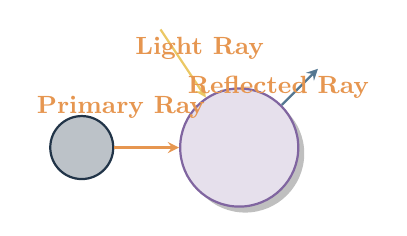
\begin{tikzpicture}[scale=0.5]
            % Simple ray tracing illustration
            \node[eye] (eye) at (0,0) {};
            \node[sphere] (sphere) at (4,0) {};
            \draw[ray] (eye) -- (sphere);
            \draw[reflectray] (sphere) -- (6,2);
            \draw[lightray] (2,3) -- (sphere);
            \node[above] at (1,0.5) {\small \raycolor{Primary Ray}};
            \node[above] at (5,1) {\small \raycolor{Reflected Ray}};
            \node[above] at (3,2) {\small \raycolor{Light Ray}};
        \end{tikzpicture}
    \end{center}
\end{frame}

% --- Table of Contents ---
\begin{frame}{Index}
    \footnotesize
    \vspace{1cm}
    \tableofcontents
\end{frame}

% --- Section 1: The Story Begins ---
\section{The Story of Light}

\begin{frame}{How Do We See?}
    \begin{columns}
        \begin{column}{0.5\textwidth}
            \begin{tikzpicture}[scale=0.8]
                % Sun
                \node[circle, fill=LightColor, minimum size=1cm] (sun) at (0,3) {\faIcon{sun}};
                \node[below] at (0,4.25) {\small \textcolor{LightColor}{Light Source}};
                \draw[lightray] (sun) -- (2,1);
                \draw[lightray] (sun) -- (3,2);
                \draw[lightray] (sun) -- (4,1);
                
                % Object
                \node[sphere] (obj) at (3,1) {};
                
                % Eye
                \node[eye] (eye) at (5,3) {\faIcon{eye}};
                \draw[reflectray] (3.1,2) -- (eye);
                
                \node[below] at (3,0) {\small \objectcolor{Object}};
                \node[below] at (5,4.1) {\small \textcolor{PrimaryColor}{Observer}};
            \end{tikzpicture}
        \end{column}
        \pause
        \begin{column}{0.5\textwidth}

            \only<2>{
                \begin{conceptbox}{Natural Process}
                    \begin{enumerate}
                        \item Light travels from source 
                        \item Light hits objects
                        \item Light bounces to our eyes
                        \item Our brain interprets the signal
                    \end{enumerate}
                \end{conceptbox}
            }

            \only<3>{
                \begin{conceptbox}{Physical Process}
                    \begin{enumerate}
                        \footnotesize 
                        \item Photon is emitted from source 
                        \item Photon hits objects
                        \item Part of the photon is reflected or absorbed
                        \item The reflected photons reach our eyes
                        \item The rods and cones in our retina detect the photons
                        \item Our brain interprets the signal
                        \item \textbf{Colour}: The wavelength of the photons
                        \item \textbf{Brightness}: The number of photons
                    \end{enumerate}
                \end{conceptbox}
            }

            \only<4>{
                \vspace{0.5cm}
                \alert{Question:} How do we simulate this?
            }

        \end{column}
    \end{columns}
\end{frame}

\begin{frame}{The Computer Graphics Challenge}
    \begin{center}
        \begin{tikzpicture}[scale=0.9]
            % Real world
            \node[rectangle, draw, minimum width=3cm, minimum height=2cm, fill=LightGray] (real) at (0,0) {\faIcon{globe} Real World};
            \node[above] at (0,1.5) {\textbf{Infinite Complexity}};
            
            % Computer
            \node[rectangle, draw, minimum width=3cm, minimum height=2cm, fill=PrimaryColor!20] (comp) at (5,0) {\faIcon{laptop} Computer};
            \node[above] at (5,1.5) {\textbf{Finite Pixels}};

            % Arrow
            \draw[->, very thick, AccentColor]
            (real.east) -- (comp.west)
            node[midway, above, text=AccentColor, font=\footnotesize]{Simulate};

            
            % Challenges
            \node[below] at (2.5,-2  ) {
                \begin{minipage}{6cm}
                    \textcolor{AccentColor}{\textbf{Challenges:}}
                    \begin{itemize}
                        \item Infinite light rays/photons
                        \item Complex physics
                        \item High computational cost
                    \end{itemize}
                \end{minipage}
            };
        \end{tikzpicture}
    \end{center}
\end{frame}

% --- Section 2: Ray Casting ---
\section{Ray Casting: Foundation}

\begin{frame}{The Key Insight}
    \begin{columns}
        \begin{column}{0.5\textwidth}
            \begin{raybox}{1. Reverse Engineering}
                Instead of following light rays from light sources |

                \vspace{0.1cm}
                \textbf{Let's trace backwards!}

                \textbf{Shoot rays from the eye}, find where it hits and find out how much light reaches there.
            \end{raybox}
            
            \vspace{0.3cm}
            This is the opposite of what happens in reality.
            \textbf{Why does this work?}
            \begin{itemize}
                \small
                \item<2-> Most light never reaches our eyes
                \item<3-> Only trace rays that matter
                \item<3-> Much more efficient!
            \end{itemize}
        \end{column}
        \begin{column}{0.5\textwidth}
            \begin{tikzpicture}[scale=0.6]
                % Define 3D styles
                \tikzset{
                    screen/.style={fill=blue!10, draw=blue!50, opacity=0.8},
                    pixel/.style={fill=AccentColor!60, thick},
                    primary ray/.style={->, very thick, red!90},
                    object/.style={fill=orange!60, draw=orange!80, circle, minimum size=12pt}
                }
                
                % Eye position in 3D space
                
                \node[eye] (eye) at (0,0,0) {\faIcon{eye}};
                % Object in 3D space
                \node[sphere, minimum size=1cm] (obj) at (8,0,3.8) {};            
                
                % Labels
                \node[below] at (0,-0.6,0) {\small Eye};
                \node[below] at (8,-1,3.8) {\small \objectcolor{Object}};

                \node[circle, fill=LightColor, minimum size=1cm] (sun) at (5,3.5) {\faIcon{sun}};
                \node[below] at (5,5) {\small \textcolor{LightColor}{Light Source}};

                \draw[ray, very thick] (eye.center) -- (obj.west);
                \draw[ray, thick, opacity=0.5] (obj.west) -- ($(sun.south) + (0,0,0)$);
                \draw[ray, thick, opacity=0.5] (obj.west) -- ($(sun.south) + (0,-0.2,-1)$);
                \draw[ray, thick, opacity=0.5] (obj.west) -- ($(sun.south) + (0,-0.3,-2)$);
                \draw[ray, thick, opacity=0.5] (obj.west) -- ($(sun.south) + (0,0.5,1)$);
                \draw[ray, thick, opacity=0.5] (obj.west) -- ($(sun.south) + (0,1.2,2)$);


                \pause

                \only<2> {
                    \draw[ray, black!50, thick, opacity=0.8, dashed] (sun) -- (obj.north);
                    \draw[ray, black!50, thick, opacity=0.8, dashed] (obj.north) -- (8,2) 
                        node[above] {\small \textcolor{black!50}{Useless ray}};
                }

                \pause 
                
            \end{tikzpicture}
        \end{column}
    \end{columns}
\end{frame}


\begin{frame}{From Infinite Rays to Finite Pixels}
    \begin{columns}
        \begin{column}{0.6\textwidth}
            \begin{raybox}{2. Cutting Costs}
                Instead of tracing infinite rays |

                \vspace{0.1cm}
                \textbf{Trace one ray per pixel.}
            \end{raybox}
            \vspace{0.3cm}
            This comes with little tradeoff, because:
            \begin{itemize}
                \small
                \item<2-> An image is just a grid of pixels
                \item<3-> Each pixel can only be of one color
                \item<4-> In the end, we just need to know the \emph{color of each pixel}
                \item<5-> Hence, one ray from the mid-point of each pixel should be a good approximation$^*$ \\                 
            \end{itemize}
            \vspace{0.3cm}
            \begin{itemize}
                \footnotesize
                \item[$^*$] We will discuss more advanced techniques later that improve quality
            \end{itemize}
        \end{column}
        \begin{column}{0.4\textwidth}
            \centering
            \pause
            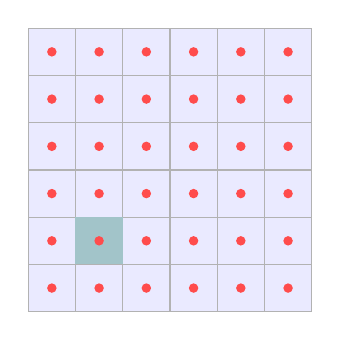
\begin{tikzpicture}[scale=0.6]
                % Define 3D styles
                \tikzset{
                    screen/.style={fill=blue!10, draw=blue!50, opacity=0.8},
                    pixel/.style={fill=AccentColor!60, thick},
                    primary ray/.style={->, very thick, red!90},
                    object/.style={fill=orange!60, draw=orange!80, circle, minimum size=12pt}
                }
            
                    \fill[screen] (-3,-3) rectangle (3,3);

                    
                    \foreach \x in {-3,-2,...,3} {
                        \draw[gray!60, thin] (\x,-3) -- (\x,3);
                    }
                    \foreach \z in {-3,-2,...,3} {
                        \draw[gray!60, thin] (-3,\z) -- (3,\z);
                    }


                    \pause
                    \fill[pixel] (-2,-2) rectangle (-1,-1);

                    \pause 
                    \pause
                    
                    \foreach \x in {-2.5,-1.5,...,2.5} {
                        \foreach \z in {-2.5,-1.5,...,2.5} {
                             \fill[red!70] (\x, \z) circle (0.1);
                        }
                    }


            \end{tikzpicture}
        \end{column}
    \end{columns}
\end{frame}


\begin{frame}{The Full Picture}
    \begin{columns}
        \begin{column}{0.5\textwidth}
            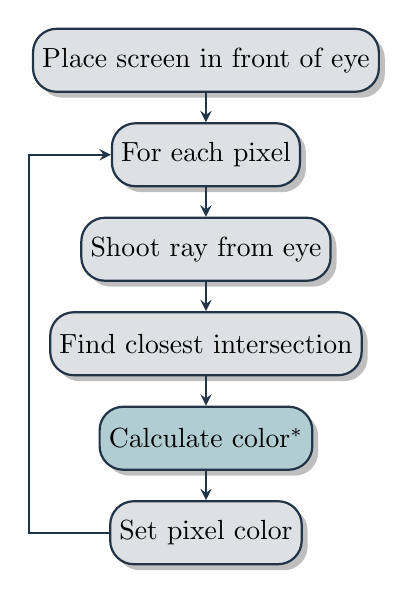
\begin{tikzpicture}[node distance=1.2cm]
                \node<2->[process] (screen) {Place screen in front of eye};
                \node<3->[process, below of=screen] (start) {For each pixel};
                \draw<3->[arrow] (screen) -- (start);

                \node<4->[process, below of=start] (ray) {Shoot ray from eye};
                \draw<4->[arrow] (start) -- (ray);

                \node<5->[process, below of=ray] (intersect) {Find closest intersection};
                \draw<5->[arrow] (ray) -- (intersect);

                \node<6->[process, fill=AccentColor!50, below of=intersect] (shade) {Calculate color$^*$};
                \draw<6->[arrow] (intersect) -- (shade);
                
                \node<7->[process, below of=shade] (end) {Set pixel color};
                \draw<7->[arrow] (shade) -- (end);
                
    
                \draw<8->[arrow] (end) -- ($(end)+(-2.25,0)$) |- (start);
                
            \end{tikzpicture}
        \end{column}
        \begin{column}{0.5\textwidth}
            \begin{tikzpicture}[scale=0.6]
                % Define 3D styles
                \tikzset{
                    screen/.style={fill=blue!10, draw=blue!50, opacity=0.8},
                    pixel/.style={fill=AccentColor!60, thick},
                    primary ray/.style={->, very thick, red!90},
                    object/.style={fill=orange!60, draw=orange!80, circle, minimum size=12pt}
                }
                
                % Eye position in 3D space
                
                \node[eye] (eye) at (0,0,0) {\faIcon{eye}};
                % Object in 3D space
                \node[sphere, minimum size=1cm] (obj) at (8,0,3.8) {};            
                
                % Labels
                \node[below] at (0,-0.6,0) {\small Eye};
                \node[below] at (8,-1,3.8) {\small \objectcolor{Object}};

                \node[circle, fill=LightColor, minimum size=1cm] (sun) at (5,3.5) {\faIcon{sun}};
                \node[below] at (5,5) {\small \textcolor{LightColor}{Light Source}};

                \pause 
                
                \node[below] at (3.5,-4,0) {\small Screen};

                \only<6->{
                    \draw[ray, thick, opacity=0.3] (obj.west) -- ($(sun.south) + (0,0,0)$);
                    \draw[ray, thick, opacity=0.3] (obj.west) -- ($(sun.south) + (0,-0.2,-1)$);
                    \draw[ray, thick, opacity=0.3] (obj.west) -- ($(sun.south) + (0,-0.3,-2)$);
                    \draw[ray, thick, opacity=0.3] (obj.west) -- ($(sun.south) + (0,0.5,1)$);
                    \draw[ray, thick, opacity=0.3] (obj.west) -- ($(sun.south) + (0,1.2,2)$);
                }


                % Screen plane in 3D (using canvas is plane)
                \begin{scope}[canvas is zy plane at x=3.5]
                    % Background screen
                    \fill[screen] (-3,-3) rectangle (3,3);

                    
                    \foreach \x in {-3,-2,...,3} {
                        \draw[gray!60, thin] (\x,-3) -- (\x,3);
                    }
                    \foreach \z in {-3,-2,...,3} {
                        \draw[gray!60, thin] (-3,\z) -- (3,\z);
                    }


                    \pause


                    \fill[pixel] (-2,-2) rectangle (-1,-1);

                    \pause 
                    \fill[red!70] (-1.5, -1.5) circle (0.1);
                    \draw<5->[ray, very thick] (eye.center) -- (-1.5, -1.5);
                    \draw<5->[->, ray, very thick] (-1.5, -1.5) -- (obj);

                    \pause
                    \pause
                    \pause 


                    \fill[RayColor!60] (-2,-2) rectangle (-1,-1);
                    \fill[red!70] (-1.5, -1.5) circle (0.1);

                    \pause

                    \foreach \x in {-2.5,-1.5,...,2.5} {
                        \foreach \z in {-2.5,-1.5,...,2.5} {
                             \fill[red!70] (\x, \z) circle (0.1);
                             \draw[ray, thick, opacity=0.3] (eye.center) -- (\x,\z);
                        }
                    }


                \end{scope}


                \draw<4>[->, ray, very thick] (eye) -- ($(obj) + (3.5, 0, 1.5)$);



                
            \end{tikzpicture}
        \end{column}
    \end{columns}
\end{frame}


\begin{frame}{Questions \& Discussion}
  \begin{center}
    \Huge \textcolor{PrimaryColor}{Questions?}

    \vspace{1cm}

    \begin{tikzpicture}
      % Decorative lighting setup
      \node[circle, fill=LightColor, minimum size=1cm] (light1) at (-2,2) {\faIcon{lightbulb}};
      \node[circle, fill=LightColor, minimum size=1cm] (light2) at (2,2) {\faIcon{lightbulb}};

      % Central question icon with Phong lighting effect
      \node[circle, fill=AccentColor!20, minimum size=3cm, drop shadow] at (0,0) {\Huge \faIcon{question}};

      % Light rays
      \foreach \angle in {-30,-15,0,15,30} {
        \draw[lightray, opacity=0.6] (light1) -- ++(\angle+45:2.5);
        \draw[lightray, opacity=0.6] (light2) -- ++(\angle+135:2.5);
      }
    \end{tikzpicture}

    \vspace{1cm}

    \Large \textcolor{SecondaryColor}{Thank you for your attention!}

    \vspace{0.5cm}

    \begin{minipage}{0.8\textwidth}
      \centering
      \footnotesize
      \textcolor{DarkGray}{
        Now you have the tools to implement realistic lighting!\\
        Practice with different materials and light setups.
      }
    \end{minipage}
  \end{center}
\end{frame}

\section{References \& Further Reading}

\begin{frame}
\frametitle{Essential References}

\begin{mathbox}{Foundational Texts}
\begin{itemize}
    \item \textbf{Real-Time Rendering, 4th Edition} \\
          Akenine-Möller, Haines, Hoffman, et al. (2018)
    \item \textbf{Computer Graphics: Principles and Practice, 3rd Edition} \\
          Hughes, van Dam, McGuire, et al. (2013)
    \item \textbf{Fundamentals of Computer Graphics, 5th Edition} \\
          Marschner \& Shirley (2021)
\end{itemize}
\end{mathbox}

\begin{conceptbox}{GPU Architecture \& Programming}
\begin{itemize}
    \item \textbf{GPU Gems Series} - NVIDIA (Free online)
    \item \textbf{GPU Pro Series} - Annual collection of advanced techniques
    \item \textbf{Graphics Programming and Shaders} - Bailey \& Cunningham
    \item \textbf{OpenGL Programming Guide} - The Khronos Group
\end{itemize}
\end{conceptbox}

\end{frame}

\begin{frame}
\frametitle{Online Resources}

\begin{conceptbox}{Documentation \& Specifications}
\begin{itemize}
    \item \textbf{OpenGL Specification}: \url{https://www.opengl.org/}
    \item \textbf{Vulkan Specification}: \url{https://www.vulkan.org/}
    \item \textbf{DirectX Documentation}: \url{https://docs.microsoft.com/en-us/windows/win32/direct3d}
    \item \textbf{WebGL Specification}: \url{https://www.khronos.org/webgl/}
\end{itemize}
\end{conceptbox}

\begin{mathbox}{Learning Resources}
\begin{itemize}
    \item \textbf{LearnOpenGL}: \url{https://learnopengl.com/}
    \item \textbf{Scratchapixel}: \url{https://www.scratchapixel.com/}
    \item \textbf{Inigo Quilez}: \url{https://iquilezles.org/}
    \item \textbf{Simon's Graphics Blog}: \url{https://simonschreibt.de/}
\end{itemize}
\end{conceptbox}

\end{frame}

\begin{frame}
\frametitle{Academic Papers \& Research}

\begin{mathbox}{Foundational Papers}
\begin{itemize}
    \item \textbf{A Hidden-Surface Algorithm with Anti-Aliasing} \\
          Catmull (1974) - Z-buffer algorithm
    \item \textbf{The A-buffer, an antialiased hidden surface method} \\
          Carpenter (1984) - Anti-aliasing techniques
    \item \textbf{Reality Engine Graphics} \\
          Akeley (1993) - Hardware rasterization
    \item \textbf{WireGL: A Scalable Graphics System for Clusters} \\
          Humphreys et al. (2001) - Distributed rendering
\end{itemize}
\end{mathbox}

\begin{conceptbox}{Modern Techniques}
\begin{itemize}
    \item \textbf{Deferred Shading} - Saito \& Takahashi (1990)
    \item \textbf{Cascaded Shadow Maps} - Zhang et al. (2006)
    \item \textbf{Screen Space Ambient Occlusion} - Mittring (2007)
    \item \textbf{Temporal Anti-Aliasing} - Yang et al. (2009)
\end{itemize}
\end{conceptbox}

\end{frame}

\begin{frame}
\frametitle{Industry Resources}

\begin{conceptbox}{Hardware Vendor Resources}
\begin{itemize}
    \item \textbf{NVIDIA Developer}: \url{https://developer.nvidia.com/}
          \begin{itemize}
              \item CUDA Programming Guide
              \item RTX Developer Resources
              \item Nsight Graphics Documentation
          \end{itemize}
    \item \textbf{AMD Developer Central}: \url{https://gpuopen.com/}
          \begin{itemize}
              \item Radeon GPU Analyzer
              \item FidelityFX SDK
              \item Performance Optimization Guides
          \end{itemize}
    \item \textbf{Intel Graphics Developers}: \url{https://www.intel.com/content/www/us/en/developer/}
          \begin{itemize}
              \item Graphics Performance Analyzers
              \item oneAPI Toolkit
          \end{itemize}
\end{itemize}
\end{conceptbox}

\end{frame}

\begin{frame}
\frametitle{Tools \& Software}

\begin{mathbox}{Graphics Debugging \& Profiling}
\begin{itemize}
    \item \textbf{RenderDoc}: Free, open-source graphics debugger
    \item \textbf{NVIDIA Nsight Graphics}: Advanced GPU debugging
    \item \textbf{AMD Radeon GPU Profiler}: Performance analysis
    \item \textbf{Intel Graphics Performance Analyzers}: Cross-platform profiling
    \item \textbf{Xcode GPU Debugger}: Metal debugging on macOS/iOS
\end{itemize}
\end{mathbox}

\begin{conceptbox}{Development Frameworks}
\begin{itemize}
    \item \textbf{OpenGL}: Cross-platform graphics API
    \item \textbf{Vulkan}: Low-level, high-performance API
    \item \textbf{Direct3D}: Microsoft's graphics API
    \item \textbf{Metal}: Apple's graphics and compute API
    \item \textbf{WebGL/WebGPU}: Browser-based graphics
\end{itemize}
\end{conceptbox}

\end{frame}

\begin{frame}
\frametitle{Conferences \& Communities}

\begin{conceptbox}{Major Conferences}
\begin{itemize}
    \item \textbf{SIGGRAPH}: Premier computer graphics conference
    \item \textbf{GDC}: Game Developers Conference
    \item \textbf{High Performance Graphics (HPG)}: Academic rendering research
    \item \textbf{Eurographics}: European computer graphics conference
    \item \textbf{I3D}: Interactive 3D Graphics and Games
\end{itemize}
\end{conceptbox}

\begin{mathbox}{Online Communities}
\begin{itemize}
    \item \textbf{Graphics Programming Discord/Reddit}: Active communities
    \item \textbf{Shadertoy}: \url{https://www.shadertoy.com/} - Shader playground
    \item \textbf{GitHub}: Open-source graphics projects and demos
    \item \textbf{Stack Overflow}: Q\&A for specific technical issues
    \item \textbf{Graphics Programming Weekly}: Curated news and resources
\end{itemize}
\end{mathbox}

\end{frame}

\begin{frame}
\frametitle{Recommended Learning Path}

\begin{center}
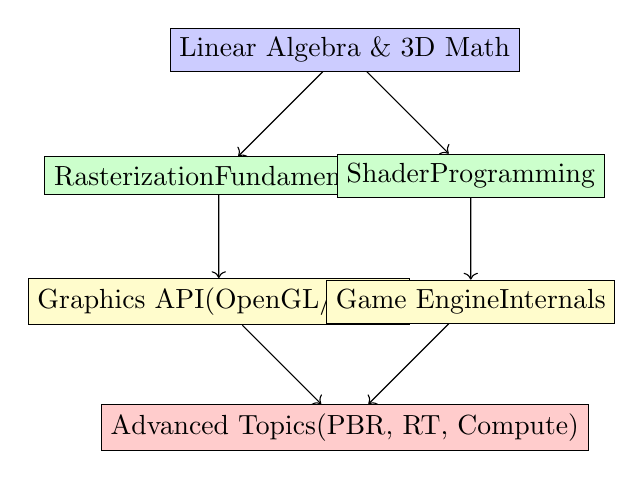
\begin{tikzpicture}[scale=0.8]
    % Learning path flowchart
    \node[draw, rectangle, fill=blue!20] (basics) at (0,4) {Linear Algebra \& 3D Math};
    
    \node[draw, rectangle, fill=green!20] (raster) at (-2,2) {Rasterization \\ Fundamentals};
    \node[draw, rectangle, fill=green!20] (shaders) at (2,2) {Shader \\ Programming};
    
    \node[draw, rectangle, fill=yellow!20] (api) at (-2,0) {Graphics API \\ (OpenGL/D3D)};
    \node[draw, rectangle, fill=yellow!20] (engine) at (2,0) {Game Engine \\ Internals};
    
    \node[draw, rectangle, fill=red!20] (advanced) at (0,-2) {Advanced Topics \\ (PBR, RT, Compute)};
    
    \draw[->] (basics) -- (raster);
    \draw[->] (basics) -- (shaders);
    \draw[->] (raster) -- (api);
    \draw[->] (shaders) -- (engine);
    \draw[->] (api) -- (advanced);
    \draw[->] (engine) -- (advanced);
\end{tikzpicture}
\end{center}

\begin{conceptbox}{Practice Projects}
\begin{enumerate}
    \item Software rasterizer implementation
    \item Simple OpenGL/Vulkan renderer
    \item Deferred rendering pipeline
    \item Shadow mapping techniques
    \item Post-processing effects
\end{enumerate}
\end{conceptbox}

\end{frame}


\end{document}
\endinput

% --- Section 3: Mathematical Foundation ---
\section{The Mathematics of Rays}

\begin{frame}{What is a Ray?}
    \begin{columns}
        \begin{column}{0.5\textwidth}
            \begin{mathbox}{Ray Representation}
                A ray is defined by:
                \begin{align}
                    \mathbf{P}(t) &= \mathbf{R_o} + t \cdot \mathbf{R_d}
                \end{align}
                where:
                \begin{itemize}
                    \item $\mathbf{R_o}$ = Origin point
                    \item $\mathbf{R_d}$ = Direction vector
                    \item $t$ = Parameter ($t \geq 0$)
                \end{itemize}
            \end{mathbox}
        \end{column}
        \begin{column}{0.5\textwidth}
            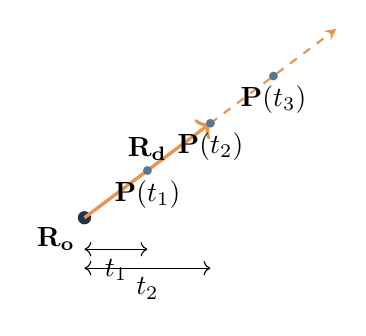
\begin{tikzpicture}[scale=0.8]
                % Origin
                \fill[PrimaryColor] (0,0) circle (3pt);
                \node[below left] at (0,0) {$\mathbf{R_o}$};
                
                % Direction vector
                \draw[->, very thick, RayColor] (0,0) -- (2,1.5);
                \node[above] at (1,0.75) {$\mathbf{R_d}$};
                
                % Ray continuation
                \draw[ray, dashed] (2,1.5) -- (4,3);
                
                % Points on ray
                \fill[SecondaryColor] (1,0.75) circle (2pt);
                \node[below] at (1,0.75) {$\mathbf{P}(t_1)$};
                \fill[SecondaryColor] (2,1.5) circle (2pt);
                \node[below] at (2,1.5) {$\mathbf{P}(t_2)$};
                \fill[SecondaryColor] (3,2.25) circle (2pt);
                \node[below] at (3,2.25) {$\mathbf{P}(t_3)$};
                
                % Parameter illustration
                \draw[<->, thin] (0,-0.5) -- (1,-0.5);
                \node[below] at (0.5,-0.5) {$t_1$};
                \draw[<->, thin] (0,-0.8) -- (2,-0.8);
                \node[below] at (1,-0.8) {$t_2$};
            \end{tikzpicture}
        \end{column}
    \end{columns}
\end{frame}

\begin{frame}{Camera and Ray Generation}
    \begin{center}
        \begin{tikzpicture}[scale=0.9]
            % Camera/Eye
            \node[eye] (eye) at (0,0) {\faIcon{camera}};
            \node[below] at (0,-0.8) {\textcolor{PrimaryColor}{Camera}};
            
            % Image plane
            \draw[thick, AccentColor] (3,-2) -- (3,2);
            \node[right] at (3,2.3) {\textcolor{AccentColor}{Image Plane}};
            
            % Pixel grid
            \foreach \y in {-1.5,-1,-0.5,0,0.5,1,1.5} {
                \draw[thin, gray] (2.8,\y) -- (3.2,\y);
            }
            
            % Sample rays
            \draw[ray] (eye) -- (3,1.5);
            \draw[ray] (eye) -- (3,0.5);
            \draw[ray] (eye) -- (3,-0.5);
            \draw[ray] (eye) -- (3,-1.5);
            
            % Objects in scene
            \node[sphere] (sphere1) at (6,1) {};
            \node[sphere] (sphere2) at (5.5,-1) {};
            \node[triangle] (tri) at (7,0) {};
            
            % Extend rays to objects
            \draw[ray, dashed] (3,1.5) -- (sphere1);
            \draw[ray, dashed] (3,-1.5) -- (sphere2);
            
            % Coordinate system
            \draw[<->, thin] (0,3) -- (0,0) -- (3,0);
            \node[left] at (0,1.5) {$v$};
            \node[below] at (1.5,0) {$u$};
            \node[below left] at (0,0) {$w$};
        \end{tikzpicture}
    \end{center}
    
    \begin{conceptbox}{Camera Parameters}
        \textbf{Camera Definition:} Eye point $\mathbf{e}$, orthobasis $\{\mathbf{u}, \mathbf{v}, \mathbf{w}\}$, field of view, image dimensions
    \end{conceptbox}
\end{frame}

% --- Section 4: Camera Models ---
\section{Camera Models in Ray Tracing}

\begin{frame}{Why Camera Models Matter}
    \begin{columns}
        \begin{column}{0.5\textwidth}
            \begin{conceptbox}{The Camera's Role}
                The camera determines:
                \begin{itemize}
                    \item \textbf{Field of view} - What we see
                    \item \textbf{Perspective} - How objects appear
                    \item \textbf{Ray generation} - Where rays start
                    \item \textbf{Image formation} - Final rendering
                \end{itemize}
            \end{conceptbox}
        \end{column}
        \begin{column}{0.5\textwidth}
            \begin{tikzpicture}[scale=0.8]
                % Camera
                \node[eye] (cam) at (0,0) {\faIcon{camera}};
                \node[below] at (0,-0.8) {\textcolor{PrimaryColor}{Camera}};
                
                % Field of view cone
                \draw[ray, fill=PrimaryColor!10] (0,0) -- (3,1.5) -- (3,-1.5) -- cycle;
                \node[right] at (3,0) {\small FOV};
                
                % Objects at different distances
                \node[sphere] (near) at (2,0.5) {};
                \node[sphere] (far) at (4,0) {};
                \node[above] at (2,1) {\tiny Near};
                \node[above] at (4,0.5) {\tiny Far};
                
                % Image plane
                \draw[thick, AccentColor] (1.5,-1) -- (1.5,1);
                \node[right] at (1.5,1.2) {\tiny Image};
            \end{tikzpicture}
        \end{column}
    \end{columns}
    
    \vspace{0.5cm}
    \begin{center}
        \alert{Different camera models = Different visual effects!}
    \end{center}
\end{frame}

\begin{frame}{The Pinhole Camera Model}
    \begin{columns}
        \begin{column}{0.5\textwidth}
            \begin{mathbox}{Pinhole Camera}
                \textbf{Key Properties:}
                \begin{itemize}
                    \item Point aperture (no lens)
                    \item Perfect focus everywhere
                    \item Linear perspective
                    \item No depth of field
                \end{itemize}
                
                \vspace{0.3cm}
                \textbf{Ray Generation:}
                \begin{align}
                    \mathbf{R_o} &= \mathbf{eye}\\
                    \mathbf{R_d} &= \mathbf{pixel} - \mathbf{eye}
                \end{align}
            \end{mathbox}
        \end{column}
        \begin{column}{0.5\textwidth}
            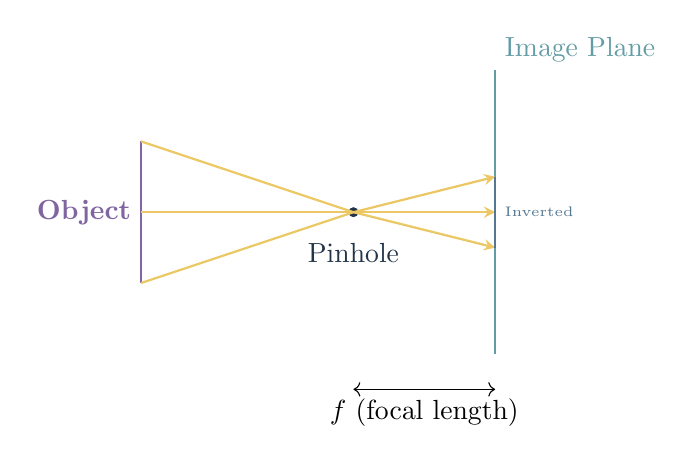
\begin{tikzpicture}[scale=0.9]
                % Pinhole
                \fill[PrimaryColor] (0,0) circle (2pt);
                \node[below] at (0,-0.3) {\textcolor{PrimaryColor}{Pinhole}};
                
                % Image plane
                \draw[thick, AccentColor] (2,-2) -- (2,2);
                \node[right] at (2,2.3) {\textcolor{AccentColor}{Image Plane}};
                
                % Object
                \draw[thick, ObjectColor] (-3,1) -- (-3,-1);
                \node[left] at (-3,0) {\objectcolor{Object}};
                
                % Light rays
                \draw[lightray] (-3,1) -- (0,0) -- (2,-0.5);
                \draw[lightray] (-3,0) -- (0,0) -- (2,0);
                \draw[lightray] (-3,-1) -- (0,0) -- (2,0.5);
                
                % Projected image
                \draw[thick, SecondaryColor] (2,-0.5) -- (2,0.5);
                \node[right] at (2,0) {\textcolor{SecondaryColor}{\tiny Inverted}};
                
                % Focal length
                \draw[<->, thin] (0,-2.5) -- (2,-2.5);
                \node[below] at (1,-2.5) {$f$ (focal length)};
            \end{tikzpicture}
        \end{column}
    \end{columns}
    
    \begin{conceptbox}{Physical Reality}
        Real pinhole cameras exist! They create sharp images but require long exposure times due to tiny aperture.
    \end{conceptbox}
\end{frame}

\begin{frame}{Simplified Pinhole Camera}
    \begin{columns}
        \begin{column}{0.5\textwidth}
            \begin{mathbox}{Simplification}
                \textbf{Problem:} Real pinhole creates inverted image
                
                \textbf{Solution:} Place image plane in front!
                \begin{align}
                    \mathbf{pixel} &= \mathbf{eye} + d \cdot \mathbf{w} + u \cdot \mathbf{u} + v \cdot \mathbf{v}
                \end{align}
                
                where:
                \begin{itemize}
                    \item $d$ = distance to image plane
                    \item $u, v$ = pixel coordinates
                    \item $\mathbf{u}, \mathbf{v}, \mathbf{w}$ = camera basis
                \end{itemize}
            \end{mathbox}
        \end{column}
        \begin{column}{0.5\textwidth}
            \begin{tikzpicture}[scale=0.9]
                % Eye/Camera
                \node[eye] (eye) at (0,0) {\faIcon{eye}};
                \node[below] at (0,-0.5) {\textcolor{PrimaryColor}{Eye}};
                
                % Image plane (in front)
                \draw[thick, AccentColor] (2,-2) -- (2,2);
                \node[right] at (2,2.3) {\textcolor{AccentColor}{Image Plane}};
                
                % Pixel grid
                \foreach \y in {-1.5,-1,-0.5,0,0.5,1,1.5} {
                    \draw[thin, gray] (1.8,\y) -- (2.2,\y);
                }
                
                % Object
                \draw[thick, ObjectColor] (4,1.5) -- (4,-1.5);
                \node[right] at (4,0) {\objectcolor{Object}};
                
                % Rays through pixels
                \draw[ray] (eye) -- (2,1.5) -- (4,1.5);
                \draw[ray] (eye) -- (2,0) -- (4,0);
                \draw[ray] (eye) -- (2,-1.5) -- (4,-1.5);
                
                % Coordinate system
                \draw[->, thin] (0,2.5) -- (0,0) -- (2.5,0);
                \node[left] at (0,1.25) {$\mathbf{v}$};
                \node[below] at (1.25,0) {$\mathbf{u}$};
                \node[above right] at (1.5,1.5) {$\mathbf{w}$};
                
                % Distance
                \draw[<->, thin] (0,-2.5) -- (2,-2.5);
                \node[below] at (1,-2.5) {$d$};
            \end{tikzpicture}
        \end{column}
    \end{columns}
    
    \begin{conceptbox}{Advantage}
        \textbf{Upright image}, easier ray generation, same perspective as real pinhole!
    \end{conceptbox}
\end{frame}

\begin{frame}{View Frustum}
    \begin{columns}
        \begin{column}{0.5\textwidth}
            \begin{mathbox}{Viewing Frustum}
                \textbf{Definition:} The 3D region visible to the camera
                
                \textbf{Boundaries:}
                \begin{itemize}
                    \item \textbf{Near plane} - Closest visible distance
                    \item \textbf{Far plane} - Farthest visible distance  
                    \item \textbf{Left/Right} - Horizontal field of view
                    \item \textbf{Top/Bottom} - Vertical field of view
                \end{itemize}
                
                \textbf{Field of View:}
                \begin{align}
                    \text{FOV} = 2 \arctan\left(\frac{h}{2d}\right)
                \end{align}
            \end{mathbox}
        \end{column}
        \begin{column}{0.5\textwidth}
            \begin{tikzpicture}[scale=0.8]
                % Camera
                \node[eye] (eye) at (0,0) {\faIcon{camera}};
                
                % Near plane
                \draw[thick, AccentColor] (1,-1) -- (1,1);
                \node[above] at (1,1.2) {\textcolor{AccentColor}{\tiny Near}};
                
                % Far plane
                \draw[thick, SecondaryColor] (4,-2) -- (4,2);
                \node[above] at (4,2.2) {\textcolor{SecondaryColor}{\tiny Far}};
                
                % Frustum edges
                \draw[ray] (eye) -- (1,1) -- (4,2);
                \draw[ray] (eye) -- (1,-1) -- (4,-2);
                \draw[ray, dashed] (eye) -- (1,0) -- (4,0);
                
                % Frustum fill
                \fill[PrimaryColor!10] (1,-1) -- (1,1) -- (4,2) -- (4,-2) -- cycle;
                
                % FOV angle
                \draw[<->, thin, bend left] (0.5,0.5) to (0.5,-0.5);
                \node[right] at (0.7,0) {\tiny FOV};
                
                % Objects inside/outside frustum
                \node[sphere] (in) at (2.5,0.5) {};
                \node[triangle] (out) at (3,-2.5) {};
                \node[above] at (2.5,1) {\tiny Visible};
                \node[below] at (3,-3) {\tiny Culled};
                
                % Distance labels
                \draw[<->, thin] (0,-2.5) -- (1,-2.5);
                \node[below] at (0.5,-2.5) {\tiny $n$};
                \draw[<->, thin] (0,-3) -- (4,-3);
                \node[below] at (2,-3) {\tiny $f$};
            \end{tikzpicture}
        \end{column}
    \end{columns}
    
    \begin{conceptbox}{Culling}
        Objects outside the frustum are \textbf{culled} (not rendered) for efficiency!
    \end{conceptbox}
\end{frame}

\begin{frame}{Orthographic Camera}
    \begin{columns}
        \begin{column}{0.5\textwidth}
            \begin{mathbox}{Orthographic Projection}
                \textbf{Key Properties:}
                \begin{itemize}
                    \item No perspective distortion
                    \item Parallel projection rays
                    \item Objects same size regardless of distance
                    \item Infinite focal length
                \end{itemize}
                
                \textbf{Ray Generation:}
                \begin{align}
                    \mathbf{R_o} &= \mathbf{pixel}\\
                    \mathbf{R_d} &= \mathbf{w} \text{ (constant)}
                \end{align}
            \end{mathbox}
        \end{column}
        \begin{column}{0.5\textwidth}
            \begin{tikzpicture}[scale=0.9]
                % Image plane
                \draw[thick, AccentColor] (0,-2) -- (0,2);
                \node[left] at (0,2.3) {\textcolor{AccentColor}{Image Plane}};
                
                % Pixel grid
                \foreach \y in {-1.5,-1,-0.5,0,0.5,1,1.5} {
                    \draw[thin, gray] (-0.2,\y) -- (0.2,\y);
                }
                
                % Object
                \draw[thick, ObjectColor] (4,1.5) -- (4,-1.5);
                \node[right] at (4,0) {\objectcolor{Object}};
                
                % Rays through pixels
                \draw[ray] (eye) -- (2,1.5) -- (4,1.5);
                \draw[ray] (eye) -- (2,0) -- (4,0);
                \draw[ray] (eye) -- (2,-1.5) -- (4,-1.5);
                
                % Coordinate system
                \draw[->, thin] (0,2.5) -- (0,0) -- (2.5,0);
                \node[left] at (0,1.25) {$\mathbf{v}$};
                \node[below] at (1.25,0) {$\mathbf{u}$};
                \node[above right] at (1.5,1.5) {$\mathbf{w}$};
                
                % Distance
                \draw[<->, thin] (0,-2.5) -- (2,-2.5);
                \node[below] at (1,-2.5) {$d$};
            \end{tikzpicture}
        \end{column}
    \end{columns}
    
    \begin{conceptbox}{Applications}
        \textbf{Technical drawings}, \textbf{CAD software}, \textbf{2D games}, architectural visualization
    \end{conceptbox}
\end{frame}

\begin{frame}{Perspective vs Orthographic}
    \begin{center}
        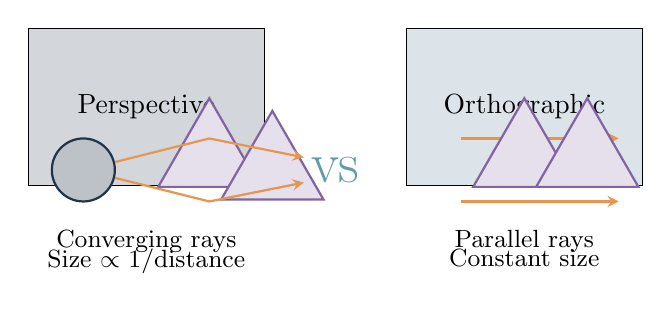
\begin{tikzpicture}[scale=0.8]
            % Perspective
            \node[rectangle, draw, minimum width=3cm, minimum height=2cm, fill=PrimaryColor!20] at (-3,2) {Perspective};
            \node[eye] (eye1) at (-4,1) {};
            \node[triangle] (near1) at (-2,1.2) {};
            \node[triangle] (far1) at (-1,1) {};
            \draw[ray] (eye1) -- (-2,1.5) -- (-0.5,1.2);
            \draw[ray] (eye1) -- (-2,0.5) -- (-0.5,0.8);
            \node[below] at (-3,0.2) {\small Converging rays};
            \node[below] at (-3,-0.1) {\small Size $\propto$ 1/distance};
            
            % vs
            \node at (0,1) {\huge \textcolor{AccentColor}{vs}};
            
            % Orthographic  
            \node[rectangle, draw, minimum width=3cm, minimum height=2cm, fill=SecondaryColor!20] at (3,2) {Orthographic};
            \draw[ray] (2,1.5) -- (4.5,1.5);
            \draw[ray] (2,0.5) -- (4.5,0.5);
            \node[triangle] (near2) at (3,1.2) {};
            \node[triangle] (far2) at (4,1.2) {};
            \node[below] at (3,0.2) {\small Parallel rays};
            \node[below] at (3,-0.1) {\small Constant size};
        \end{tikzpicture}
    \end{center}
    
    \vspace{0.5cm}
    \begin{columns}
        \begin{column}{0.5\textwidth}
            \begin{raybox}{When to use Perspective}
                \begin{itemize}
                    \item Natural/realistic scenes
                    \item Human vision simulation
                    \item Games and films
                    \item Depth perception important
                \end{itemize}
            \end{raybox}
        \end{column}
        \begin{column}{0.5\textwidth}
            \begin{raybox}{When to use Orthographic}
                \begin{itemize}
                    \item Technical illustrations
                    \item CAD/Engineering
                    \item UI elements overlay
                    \item Precise measurements
                \end{itemize}
            \end{raybox}
        \end{column}
    \end{columns}
\end{frame}

\begin{frame}{Other Camera Types}
    \begin{columns}
        \begin{column}{0.5\textwidth}
            \begin{conceptbox}{Fish-eye Camera}
                \begin{itemize}
                    \item Very wide field of view (>180°)
                    \item Non-linear distortion
                    \item Curved ray paths
                    \item Surveillance, VR applications
                \end{itemize}
            \end{conceptbox}
            
            \vspace{0.3cm}
            \begin{conceptbox}{Thin Lens Camera}
                \begin{itemize}
                    \item Simulates real camera lens
                    \item Depth of field effects
                    \item Focal blur
                    \item Aperture and focus distance
                \end{itemize}
            \end{conceptbox}
        \end{column}
        \begin{column}{0.5\textwidth}
            \begin{tikzpicture}[scale=0.8]
                % Fish-eye illustration
                \node[above] at (0,3) {\textbf{Fish-eye FOV}};
                \node[eye] (fisheye) at (0,2) {\faIcon{eye}};
                \draw[ray, bend left=30] (fisheye) to (2,3);
                \draw[ray] (fisheye) -- (2,2);
                \draw[ray, bend right=30] (fisheye) to (2,1);
                \draw[ray, bend left=60] (fisheye) to (1,3.5);
                \draw[ray, bend right=60] (fisheye) to (1,0.5);
                \node[right] at (2.2,2) {\tiny Wide FOV};
                
                % Thin lens illustration
                \node[above] at (0,0.5) {\textbf{Thin Lens}};
                \draw[thick, PrimaryColor] (-0.5,-1) -- (0.5,-1);
                \node[left] at (-0.5,-1) {\textcolor{PrimaryColor}{Lens}};
                \draw[ray] (-1,-0.5) -- (0,-1) -- (2,-1.5);
                \draw[ray] (-1,-1.5) -- (0,-1) -- (2,-0.5);
                \fill[AccentColor] (2,-1) circle (1pt);
                \node[right] at (2,-1) {\textcolor{AccentColor}{Focus}};
            \end{tikzpicture}
        \end{column}
    \end{columns}
    
    \begin{columns}
        \begin{column}{0.5\textwidth}
            \begin{conceptbox}{Environment Camera}
                \begin{itemize}
                    \item 360° panoramic view
                    \item Spherical or cylindrical
                    \item HDRI environment maps
                    \item VR content creation
                \end{itemize}
            \end{conceptbox}
        \end{column}
        \begin{column}{0.5\textwidth}
            \begin{conceptbox}{Motion Blur Camera}
                \begin{itemize}
                    \item Simulates camera/object motion
                    \item Multiple time samples
                    \item Temporal anti-aliasing
                    \item Dynamic scene rendering
                \end{itemize}
            \end{conceptbox}
        \end{column}
    \end{columns}
\end{frame}

% --- Section 5: Intersection Algorithms ---
\section{Ray-Object Intersections}

\begin{frame}{The Heart of Ray Tracing}
    \begin{center}
        \huge \textcolor{PrimaryColor}{Finding Intersections}
    \end{center}
    
    \vspace{0.5cm}
    \begin{columns}
        \begin{column}{0.5\textwidth}
            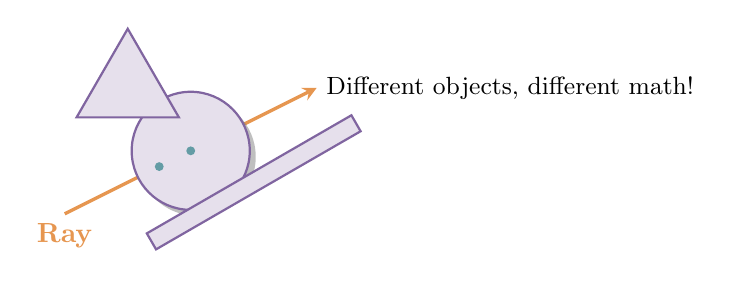
\begin{tikzpicture}[scale=0.8]
                % Ray
                \draw[ray, very thick] (0,0) -- (4,2);
                \node[below] at (0,0) {\raycolor{Ray}};
                
                % Various objects
                \node[sphere] (sphere) at (2,1) {};
                \node[plane, rotate=30] (plane) at (3,0.5) {};
                \node[triangle] (tri) at (1,2) {};
                
                % Intersection points
                \fill[AccentColor] (1.5,0.75) circle (2pt);
                \fill[AccentColor] (2,1) circle (2pt);
                
                \node[right] at (4,2) {\small Different objects, different math!};
            \end{tikzpicture}
        \end{column}
        \begin{column}{0.5\textwidth}
            \textbf{Key Objects:}
            \begin{itemize}
                \item \objectcolor{Planes} - Linear equations
                \item \objectcolor{Spheres} - Quadratic equations  
                \item \objectcolor{Triangles} - Barycentric coordinates
                \item \objectcolor{General Quadrics} - Polynomial solving
            \end{itemize}
            \vspace{0.5cm}
            \alert{Challenge:} Find the \textbf{closest} intersection efficiently!
        \end{column}
    \end{columns}
\end{frame}

\begin{frame}{Ray-Plane Intersection}
    \begin{columns}
        \begin{column}{0.5\textwidth}
            \begin{mathbox}{Plane Equation}
                Implicit form:
                \begin{align}
                    \mathbf{n} \cdot \mathbf{P} + D &= 0
                \end{align}
                
                Substituting ray equation:
                \begin{align}
                    \mathbf{n} \cdot (\mathbf{R_o} + t\mathbf{R_d}) + D &= 0\\
                    t &= -\frac{D + \mathbf{n} \cdot \mathbf{R_o}}{\mathbf{n} \cdot \mathbf{R_d}}
                \end{align}
            \end{mathbox}
        \end{column}
        \begin{column}{0.5\textwidth}
            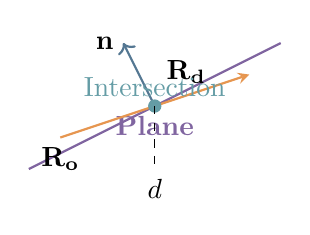
\begin{tikzpicture}[scale=0.8]
                % Plane
                \draw[thick, ObjectColor] (-1,0) -- (3,2);
                \node[below] at (1,1) {\objectcolor{Plane}};
                
                % Normal vector
                \draw[->, thick, SecondaryColor] (1,1) -- (0.5,2);
                \node[left] at (0.5,2) {$\mathbf{n}$};
                
                % Ray
                \draw[ray] (-0.5,0.5) -- (2.5,1.5);
                \node[below] at (-0.5,0.5) {$\mathbf{R_o}$};
                \node[above] at (1.5,1.2) {$\mathbf{R_d}$};
                
                % Intersection point
                \fill[AccentColor] (1,1) circle (3pt);
                \node[above] at (1,1) {\textcolor{AccentColor}{Intersection}};
                
                % Distance illustration
                \draw[dashed, thin] (1,1) -- (1,0);
                \node[below] at (1,0) {$d$};
            \end{tikzpicture}
        \end{column}
    \end{columns}
    
    \begin{conceptbox}{Key Insight}
        \textbf{Explicit} ray equation meets \textbf{implicit} plane equation = Clean intersection formula!
    \end{conceptbox}
\end{frame}

\begin{frame}{Ray-Sphere Intersection}
    \begin{columns}
        \begin{column}{0.5\textwidth}
            \begin{mathbox}{Sphere Equation}
                Implicit form (centered at origin):
                \begin{align}
                    \mathbf{P} \cdot \mathbf{P} - r^2 &= 0
                \end{align}
                
                Substituting ray equation:
                \begin{align}
                    &(\mathbf{R_o} + t\mathbf{R_d}) \cdot (\mathbf{R_o} + t\mathbf{R_d}) - r^2 = 0\\
                    &t^2 + 2(\mathbf{R_d} \cdot \mathbf{R_o})t + (\mathbf{R_o} \cdot \mathbf{R_o} - r^2) = 0
                \end{align}
                
                Quadratic formula: $t = \frac{-b \pm \sqrt{b^2-4ac}}{2a}$
            \end{mathbox}
        \end{column}
        \begin{column}{0.5\textwidth}
            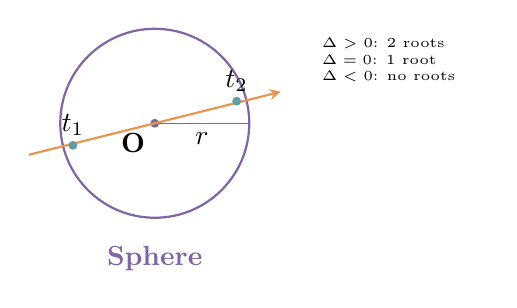
\begin{tikzpicture}[scale=0.8]
                % Sphere
                \draw[thick, ObjectColor] (0,0) circle (1.5);
                \node[below] at (0,-1.8) {\objectcolor{Sphere}};
                
                % Center
                \fill[ObjectColor] (0,0) circle (2pt);
                \node[below left] at (0,0) {$\mathbf{O}$};
                
                % Radius
                \draw[thin, ObjectColor] (0,0) -- (1.5,0);
                \node[below] at (0.75,0) {$r$};
                
                % Ray with two intersections
                \draw[ray] (-2,-0.5) -- (2,0.5);
                
                % Intersection points
                \fill[AccentColor] (-1.3,-0.35) circle (2pt);
                \fill[AccentColor] (1.3,0.35) circle (2pt);
                \node[above] at (-1.3,-0.35) {$t_1$};
                \node[above] at (1.3,0.35) {$t_2$};
                
                % Discriminant cases
                \node[right] at (2.5,1) {
                    \begin{minipage}{2cm}
                        \tiny
                        $\Delta > 0$: 2 roots\\
                        $\Delta = 0$: 1 root\\
                        $\Delta < 0$: no roots
                    \end{minipage}
                };
            \end{tikzpicture}
        \end{column}
    \end{columns}
\end{frame}

\begin{frame}{Ray-Triangle Intersection}
    \begin{columns}
        \begin{column}{0.5\textwidth}
            \begin{mathbox}{Barycentric Approach}
                Triangle defined by vertices $\mathbf{a}$, $\mathbf{b}$, $\mathbf{c}$:
                \begin{align}
                    \mathbf{P}(\beta,\gamma) &= \mathbf{a} + \beta(\mathbf{b}-\mathbf{a}) + \gamma(\mathbf{c}-\mathbf{a})
                \end{align}
                
                Set equal to ray equation:
                \begin{align}
                    \mathbf{R_o} + t\mathbf{R_d} &= \mathbf{a} + \beta(\mathbf{b}-\mathbf{a}) + \gamma(\mathbf{c}-\mathbf{a})
                \end{align}
                
                Solve 3×3 system for $t$, $\beta$, $\gamma$
            \end{mathbox}
        \end{column}
        \begin{column}{0.5\textwidth}
            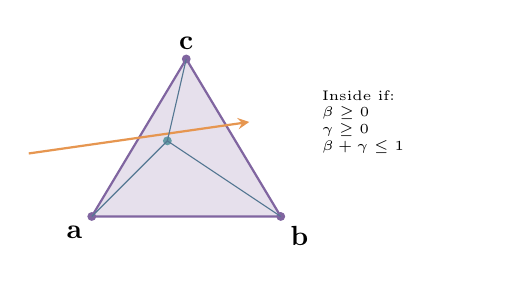
\begin{tikzpicture}[scale=0.8]
                % Triangle
                \coordinate (A) at (0,0);
                \coordinate (B) at (3,0);
                \coordinate (C) at (1.5,2.5);
                
                \draw[thick, ObjectColor, fill=ObjectColor!20] (A) -- (B) -- (C) -- cycle;
                
                % Vertices
                \fill[ObjectColor] (A) circle (2pt);
                \fill[ObjectColor] (B) circle (2pt);
                \fill[ObjectColor] (C) circle (2pt);
                \node[below left] at (A) {$\mathbf{a}$};
                \node[below right] at (B) {$\mathbf{b}$};
                \node[above] at (C) {$\mathbf{c}$};
                
                % Ray
                \draw[ray] (-1,1) -- (2.5,1.5);
                
                % Intersection point
                \fill[AccentColor] (1.2,1.2) circle (2pt);
                
                % Barycentric coordinates illustration
                \draw[thin, SecondaryColor] (A) -- (1.2,1.2);
                \draw[thin, SecondaryColor] (B) -- (1.2,1.2);
                \draw[thin, SecondaryColor] (C) -- (1.2,1.2);
                
                \node[right] at (3.5,1.5) {
                    \begin{minipage}{2cm}
                        \tiny
                        Inside if:\\
                        $\beta \geq 0$\\
                        $\gamma \geq 0$\\
                        $\beta + \gamma \leq 1$
                    \end{minipage}
                };
            \end{tikzpicture}
        \end{column}
    \end{columns}
\end{frame}

% --- Section 6: From Casting to Tracing ---
\section{From Ray Casting to Ray Tracing}

\begin{frame}{Ray Casting vs Ray Tracing}
    \begin{center}
        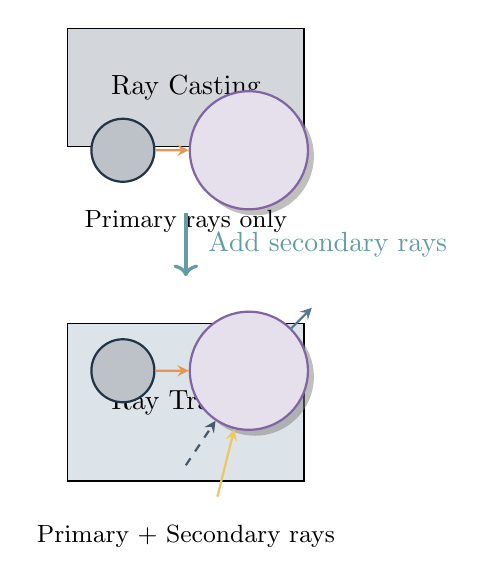
\begin{tikzpicture}[scale=0.8]
            % Ray Casting
            \node[rectangle, draw, minimum width=3cm, minimum height=1.5cm, fill=PrimaryColor!20] at (0,2) {Ray Casting};
            \node[eye] (eye1) at (-1,1) {};
            \node[sphere] (obj1) at (1,1) {};
            \draw[ray] (eye1) -- (obj1);
            \node[below] at (0,0.2) {\small Primary rays only};
            
            % Arrow
            \draw[->, very thick, AccentColor] (0,0) -- (0,-1);
            \node[right] at (0.2,-0.5) {\textcolor{AccentColor}{Add secondary rays}};
            
            % Ray Tracing
            \node[rectangle, draw, minimum width=3cm, minimum height=2cm, fill=SecondaryColor!20] at (0,-3) {Ray Tracing};
            \node[eye] (eye2) at (-1,-2.5) {};
            \node[sphere] (obj2) at (1,-2.5) {};
            \draw[ray] (eye2) -- (obj2);
            \draw[reflectray] (obj2) -- (2,-1.5);
            \draw[shadowray] (0,-4) -- (obj2);
            \draw[lightray] (0.5,-4.5) -- (obj2);
            \node[below] at (0,-4.8) {\small Primary + Secondary rays};
        \end{tikzpicture}
    \end{center}
    
    \begin{columns}
        \begin{column}{0.5\textwidth}
            \begin{raybox}{Ray Casting}
                \begin{itemize}
                    \item Eye rays only
                    \item Direct illumination
                    \item Fast but limited
                    \item Good for basic scenes
                \end{itemize}
            \end{raybox}
        \end{column}
        \begin{column}{0.5\textwidth}
            \begin{raybox}{Ray Tracing}
                \begin{itemize}
                    \item Multiple ray types
                    \item Global illumination
                    \item Slower but realistic
                    \item Reflections, shadows, refraction
                \end{itemize}
            \end{raybox}
        \end{column}
    \end{columns}
\end{frame}

\begin{frame}{Secondary Rays: The Magic Ingredients}
    \begin{center}
        \begin{tikzpicture}[scale=0.9]
            % Main scene setup
            \node[eye] (eye) at (0,0) {\faIcon{eye}};
            \node[sphere] (sphere) at (4,0) {};
            \node[circle, fill=LightColor, minimum size=0.8cm] (light) at (2,3) {\faIcon{lightbulb}};
            \node[sphere] (mirror) at (6,2) {};
            
            % Primary ray
            \draw[ray, very thick] (eye) -- (sphere);
            \node[below] at (2,-0.3) {\raycolor{1. Primary Ray}};
            
            % Shadow ray
            \draw[shadowray] (sphere) -- (light);
            \node[right] at (3.5,1.8) {\textcolor{DarkGray}{2. Shadow Ray}};
            
            % Reflection ray
            \draw[reflectray] (sphere) -- (mirror);
            \node[above] at (5,1.2) {\textcolor{SecondaryColor}{3. Reflection Ray}};
            
            % Ground plane
            \draw[thick, ObjectColor] (-1,-1.5) -- (7,-1.5);
            \draw[refractray] (sphere) -- (4,-1.5);
            \node[right] at (4.2,-1) {\textcolor{AccentColor}{4. Refraction Ray}};
            
            % Labels
            \node[above] at (2,3.5) {\textcolor{LightColor}{Light Source}};
            \node[above] at (6,2.8) {\textcolor{ObjectColor}{Mirror}};
            \node[below] at (4,-0.8) {\textcolor{ObjectColor}{Main Object}};
        \end{tikzpicture}
    \end{center}
\end{frame}

\begin{frame}{Recursive Ray Tracing}
    \begin{center}
        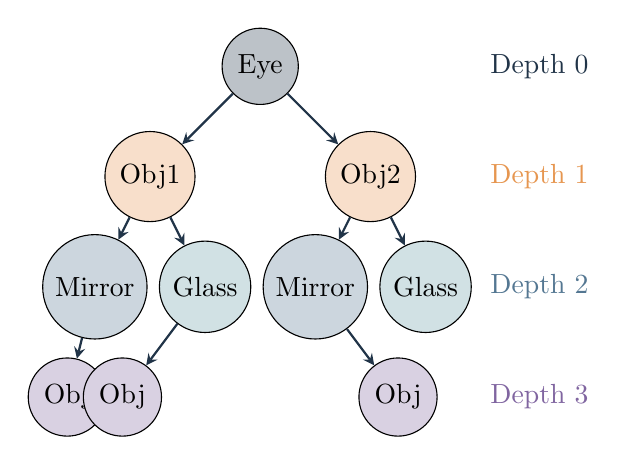
\begin{tikzpicture}[scale=0.7]
            % Tree structure showing recursion
            \node[circle, draw, fill=PrimaryColor!30] (root) at (0,4) {Eye};
            
            % Level 1
            \node[circle, draw, fill=RayColor!30] (obj1) at (-2,2) {Obj1};
            \node[circle, draw, fill=RayColor!30] (obj2) at (2,2) {Obj2};
            
            % Level 2
            \node[circle, draw, fill=SecondaryColor!30] (mirror1) at (-3,0) {Mirror};
            \node[circle, draw, fill=AccentColor!30] (glass1) at (-1,0) {Glass};
            \node[circle, draw, fill=SecondaryColor!30] (mirror2) at (1,0) {Mirror};
            \node[circle, draw, fill=AccentColor!30] (glass2) at (3,0) {Glass};
            
            % Level 3
            \node[circle, draw, fill=ObjectColor!30] (final1) at (-3.5,-2) {Obj};
            \node[circle, draw, fill=ObjectColor!30] (final2) at (-2.5,-2) {Obj};
            \node[circle, draw, fill=ObjectColor!30] (final3) at (2.5,-2) {Obj};
            
            % Connections
            \draw[arrow] (root) -- (obj1);
            \draw[arrow] (root) -- (obj2);
            \draw[arrow] (obj1) -- (mirror1);
            \draw[arrow] (obj1) -- (glass1);
            \draw[arrow] (obj2) -- (mirror2);
            \draw[arrow] (obj2) -- (glass2);
            \draw[arrow] (mirror1) -- (final1);
            \draw[arrow] (glass1) -- (final2);
            \draw[arrow] (mirror2) -- (final3);
            
            % Depth labels
            \node[right] at (4,4) {\textcolor{PrimaryColor}{Depth 0}};
            \node[right] at (4,2) {\textcolor{RayColor}{Depth 1}};
            \node[right] at (4,0) {\textcolor{SecondaryColor}{Depth 2}};
            \node[right] at (4,-2) {\textcolor{ObjectColor}{Depth 3}};
        \end{tikzpicture}
    \end{center}
    
    \begin{conceptbox}{Recursion Control}
        \textbf{Base Cases:} Maximum depth reached OR ray contribution becomes negligible
    \end{conceptbox}
\end{frame}

% --- Section 7: Advanced Topics ---
\section{Advanced Ray Tracing Effects}

\begin{frame}{Mirror Reflections}
    \begin{columns}
        \begin{column}{0.5\textwidth}
            \begin{mathbox}{Reflection Law}
                Given incident ray $\mathbf{d}$ and surface normal $\mathbf{n}$:
                \begin{align}
                    \mathbf{r} &= \mathbf{d} - 2(\mathbf{d} \cdot \mathbf{n})\mathbf{n}
                \end{align}
                
                \vspace{0.5cm}
                \textbf{Physical principle:}\\
                Angle of incidence = Angle of reflection
            \end{mathbox}
        \end{column}
        \begin{column}{0.5\textwidth}
            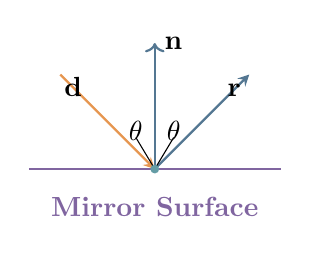
\begin{tikzpicture}[scale=0.8]
                % Mirror surface
                \draw[thick, ObjectColor] (-0.5,0) -- (3.5,0);
                \node[below] at (1.5,-0.3) {\objectcolor{Mirror Surface}};
                
                % Normal vector
                \draw[->, thick, SecondaryColor] (1.5,0) -- (1.5,2);
                \node[right] at (1.5,2) {$\mathbf{n}$};
                
                % Incident ray
                \draw[ray] (0,1.5) -- (1.5,0);
                \node[above left] at (0.5,1) {$\mathbf{d}$};
                
                % Reflected ray
                \draw[reflectray] (1.5,0) -- (3,1.5);
                \node[above right] at (2.5,1) {$\mathbf{r}$};
                
                % Angle indicators
                \draw[thin] (1.5,0) -- (1.2,0.5);
                \draw[thin] (1.5,0) -- (1.8,0.5);
                \node[above] at (1.2,0.3) {$\theta$};
                \node[above] at (1.8,0.3) {$\theta$};
                
                % Intersection point
                \fill[AccentColor] (1.5,0) circle (2pt);
            \end{tikzpicture}
        \end{column}
    \end{columns}
    
    \begin{center}
        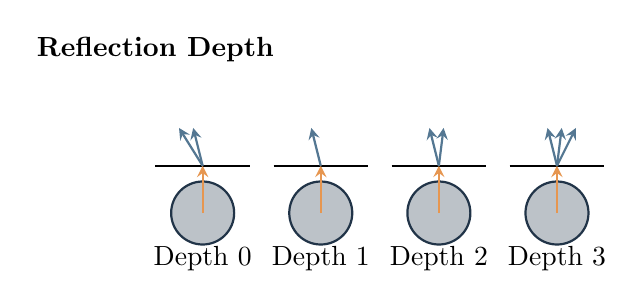
\begin{tikzpicture}[scale=0.6]
            % Depth progression
            \node[above] at (0,2) {\textbf{Reflection Depth}};
            
            \foreach \depth/\x in {0/0, 1/2.5, 2/5, 3/7.5} {
                \begin{scope}[xshift=\x cm]
                    \draw[thick] (0,0) -- (2,0);
                    \node[eye] at (1,-1) {};
                    \draw[ray] (1,-1) -- (1,0);
                    \foreach \i in {1,...,\depth} {
                        \draw[reflectray] (1,0) -- (0.5+\i*0.3,0.8);
                    }
                    \node[below] at (1,-1.5) {Depth \depth};
                \end{scope}
            }
        \end{tikzpicture}
    \end{center}
\end{frame}

\begin{frame}{Refraction and Snell's Law}
    \begin{columns}
        \begin{column}{0.5\textwidth}
            \begin{mathbox}{Snell's Law}
                \begin{align}
                    n_1 \sin\theta_1 &= n_2 \sin\theta_2
                \end{align}
                
                where:
                \begin{itemize}
                    \item $n_1, n_2$ = refractive indices
                    \item $\theta_1$ = incident angle
                    \item $\theta_2$ = refracted angle
                \end{itemize}
                
                \vspace{0.3cm}
                \textbf{Examples:}
                \begin{itemize}
                    \item Air: $n = 1.0$
                    \item Water: $n = 1.33$
                    \item Glass: $n = 1.5$
                \end{itemize}
            \end{mathbox}
        \end{column}
        \begin{column}{0.5\textwidth}
            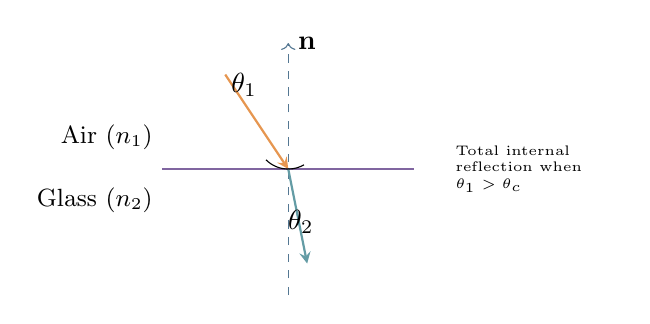
\begin{tikzpicture}[scale=0.8]
                % Interface
                \draw[thick, ObjectColor] (-1,0) -- (3,0);
                \node[left] at (-1,0.5) {\small Air ($n_1$)};
                \node[left] at (-1,-0.5) {\small Glass ($n_2$)};
                
                % Normal
                \draw[->, SecondaryColor, dashed] (1,-2) -- (1,2);
                \node[right] at (1,2) {$\mathbf{n}$};
                
                % Incident ray
                \draw[ray] (0,1.5) -- (1,0);
                \node[above] at (0.3,1) {$\theta_1$};
                
                % Refracted ray
                \draw[refractray] (1,0) -- (1.3,-1.5);
                \node[below] at (1.2,-0.5) {$\theta_2$};
                
                % Angles
                \draw[thin] (1,0) arc (270:225:0.5);
                \draw[thin] (1,0) arc (270:300:0.5);
                
                % Critical angle illustration
                \node[right] at (3.5,0) {
                    \begin{minipage}{2cm}
                        \tiny
                        Total internal\\
                        reflection when\\
                        $\theta_1 > \theta_c$
                    \end{minipage}
                };
            \end{tikzpicture}
        \end{column}
    \end{columns}
    
    \begin{conceptbox}{Physical Intuition}
        Light bends when moving between materials with different densities
    \end{conceptbox}
\end{frame}

\begin{frame}{Shadows: The Absence of Light}
    \begin{center}
        \begin{tikzpicture}[scale=0.9]
            % Light source
            \node[circle, fill=LightColor, minimum size=1cm] (light) at (0,3) {\faIcon{sun}};
            \node[above] at (0,3.8) {\textcolor{LightColor}{Light Source}};
            
            % Occluding object
            \node[sphere] (occluder) at (2,2) {};
            \node[above] at (2,2.8) {\textcolor{ObjectColor}{Occluder}};
            
            % Target object
            \node[sphere] (target) at (5,0) {};
            \node[below] at (5,-0.8) {\textcolor{ObjectColor}{Target}};
            
            % Eye
            \node[eye] (eye) at (7,0) {\faIcon{eye}};
            
            % Primary ray from eye
            \draw[ray] (eye) -- (target);
            \node[above] at (6,0.2) {\raycolor{Primary}};
            
            % Shadow ray (blocked)
            \draw[shadowray] (target) -- (occluder);
            \draw[shadowray, dashed] (occluder) -- (light);
            \node[left] at (3.5,1.2) {\textcolor{DarkGray}{Shadow Ray}};
            \node[right] at (3.5,1.5) {\textcolor{AccentColor}{BLOCKED!}};
            
            % Shadow region
            \fill[pattern=north east lines, pattern color=gray] (2.5,1.5) -- (4,0.5) -- (6,-0.5) -- (5.5,0.5) -- cycle;
            \node[right] at (6,0.8) {\textcolor{DarkGray}{Shadow}};
        \end{tikzpicture}
    \end{center}
    
    \begin{raybox}{Shadow Ray Algorithm}
        \textbf{For each intersection point:}
        \begin{enumerate}
            \item Cast ray toward each light source
            \item Check if ray intersects any object before reaching light
            \item If blocked → point is in shadow
            \item If clear → point is illuminated
        \end{enumerate}
    \end{raybox}
\end{frame}

% --- Section 8: Implementation Challenges ---
\section{Implementation Challenges}

\begin{frame}{The Floating Point Precision Problem}
    \begin{center}
        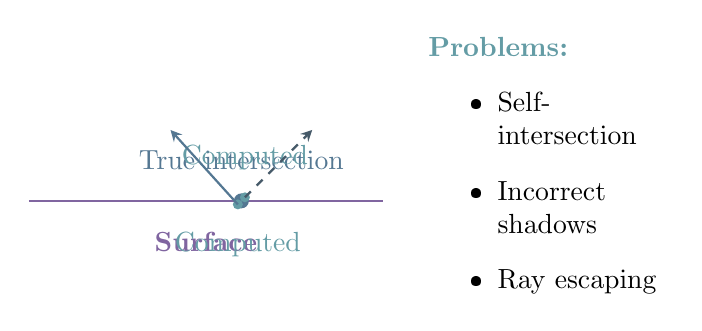
\begin{tikzpicture}[scale=0.9]
            % Surface
            \draw[thick, ObjectColor] (-1,0) -- (4,0);
            \node[below] at (1.5,-0.3) {\objectcolor{Surface}};
            
            % True intersection point
            \fill[SecondaryColor] (2,0) circle (3pt);
            \node[above] at (2,0.3) {\textcolor{SecondaryColor}{True intersection}};
            
            % Computed intersection points (with error)
            \fill[AccentColor] (1.95,-0.05) circle (2pt);
            \fill[AccentColor] (2.05,0.05) circle (2pt);
            \node[below] at (1.95,-0.3) {\textcolor{AccentColor}{Computed}};
            \node[above] at (2.05,0.3) {\textcolor{AccentColor}{Computed}};
            
            % Secondary rays from computed points
            \draw[reflectray] (1.95,-0.05) -- (1,1);
            \draw[shadowray] (2.05,0.05) -- (3,1);
            
            % Problems
            \node[right] at (4.5,0.5) {
                \begin{minipage}{3cm}
                    \textcolor{AccentColor}{\textbf{Problems:}}
                    \begin{itemize}
                        \item Self-intersection
                        \item Incorrect shadows
                        \item Ray escaping
                    \end{itemize}
                \end{minipage}
            };
        \end{tikzpicture}
    \end{center}
    
    \begin{conceptbox}{The Evil Epsilon}
        \textbf{Solution:} Add small offset $\varepsilon$ when starting secondary rays from surfaces\\
        \textbf{Challenge:} Too small → still problems; Too large → visible artifacts
    \end{conceptbox}
\end{frame}

\begin{frame}{Performance Considerations}
    \begin{columns}
        \begin{column}{0.5\textwidth}
            \begin{raybox}{Computational Complexity}
                \textbf{Basic ray tracing:}
                \begin{itemize}
                    \item $O(n \times m)$ where:
                    \item $n$ = number of pixels
                    \item $m$ = number of objects
                \end{itemize}
                
                \vspace{0.3cm}
                \textbf{With secondary rays:}
                \begin{itemize}
                    \item Exponential growth with depth
                    \item Multiple rays per intersection
                \end{itemize}
            \end{raybox}
        \end{column}
        \begin{column}{0.5\textwidth}
            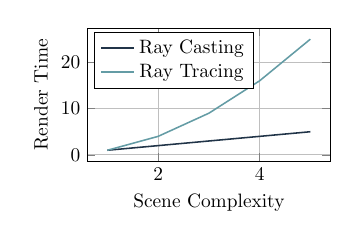
\begin{tikzpicture}[scale=0.7]
                % Performance graph
                \begin{axis}[
                    width=6cm,
                    height=4cm,
                    xlabel={Scene Complexity},
                    ylabel={Render Time},
                    grid=major,
                    legend pos=north west
                ]
                \addplot[thick, PrimaryColor] coordinates {(1,1) (2,2) (3,3) (4,4) (5,5)};
                \addplot[thick, AccentColor] coordinates {(1,1) (2,4) (3,9) (4,16) (5,25)};
                \legend{Ray Casting, Ray Tracing}
                \end{axis}
            \end{tikzpicture}
            
            \vspace{0.3cm}
            \textbf{Optimization strategies:}
            \begin{itemize}
                \item Spatial data structures
                \item Early ray termination
                \item Parallel processing
            \end{itemize}
        \end{column}
    \end{columns}
\end{frame}

% --- Section 9: Acceleration Structures ---
\section{Acceleration Structures: Making Ray Tracing Fast}

\begin{frame}{The Naive Approach Problem}
    \begin{center}
        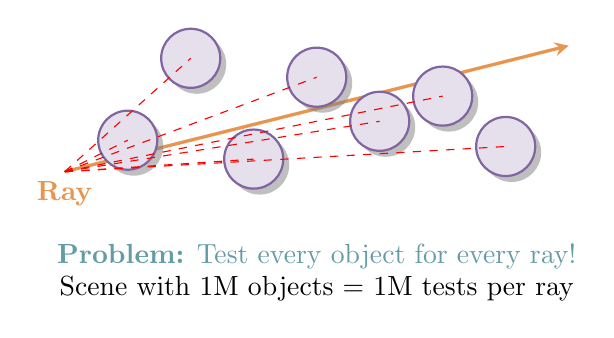
\begin{tikzpicture}[scale=0.8]
            % Ray
            \draw[ray, very thick] (0,0) -- (8,2);
            \node[below] at (0,0) {\raycolor{Ray}};
            
            % Many objects scattered
            \foreach \x/\y in {1/0.5, 2/1.8, 3/0.2, 4/1.5, 5/0.8, 6/1.2, 7/0.4} {
                \node[sphere, scale=0.5] at (\x,\y) {};
            }
            
            % Intersection tests
            \foreach \x/\y in {1/0.5, 2/1.8, 3/0.2, 4/1.5, 5/0.8, 6/1.2, 7/0.4} {
                \draw[dashed, red, thin] (0,0) -- (\x,\y);
            }
            
            \node[below] at (4,-1) {\textcolor{AccentColor}{\textbf{Problem:} Test every object for every ray!}};
            \node[below] at (4,-1.5) {Scene with 1M objects = 1M tests per ray};
        \end{tikzpicture}
    \end{center}
    
    \begin{conceptbox}{Computational Explosion}
        \textbf{Complexity:} For $N$ objects and $R$ rays → $O(N \times R)$ intersection tests\\
        \textbf{Real scenes:} Millions of triangles, millions of rays → Billions of tests!
    \end{conceptbox}
\end{frame}

\begin{frame}{Bounding Volume Hierarchy (BVH)}
    \begin{columns}
        \begin{column}{0.5\textwidth}
            \begin{raybox}{The Big Idea}
                \textbf{Divide and Conquer:}
                \begin{enumerate}
                    \item Group objects into bounding boxes
                    \item Build hierarchical tree structure
                    \item Test ray against boxes first
                    \item Only test objects in hit boxes
                \end{enumerate}
            \end{raybox}
            
            \vspace{0.3cm}
            \textbf{Key Benefits:}
            \begin{itemize}
                \item $O(\log N)$ instead of $O(N)$
                \item Massive speedup for complex scenes
                \item Works with any primitive type
            \end{itemize}
        \end{column}
        \begin{column}{0.5\textwidth}
            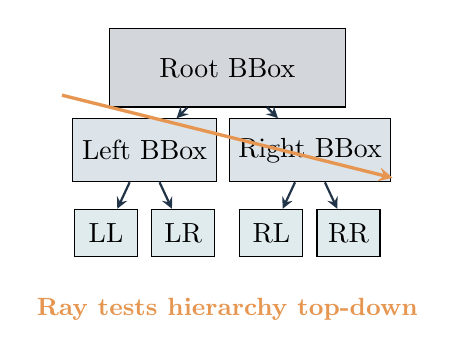
\begin{tikzpicture}[scale=0.7]
                % BVH Tree structure
                \node[rectangle, draw, fill=PrimaryColor!20, minimum width=3cm, minimum height=1cm] (root) at (0,3) {Root BBox};
                
                \node[rectangle, draw, fill=SecondaryColor!20, minimum width=1.3cm, minimum height=0.8cm] (left) at (-1.5,1.5) {Left BBox};
                \node[rectangle, draw, fill=SecondaryColor!20, minimum width=1.3cm, minimum height=0.8cm] (right) at (1.5,1.5) {Right BBox};
                
                \node[rectangle, draw, fill=AccentColor!20, minimum width=0.8cm, minimum height=0.6cm] (ll) at (-2.2,0) {LL};
                \node[rectangle, draw, fill=AccentColor!20, minimum width=0.8cm, minimum height=0.6cm] (lr) at (-0.8,0) {LR};
                \node[rectangle, draw, fill=AccentColor!20, minimum width=0.8cm, minimum height=0.6cm] (rl) at (0.8,0) {RL};
                \node[rectangle, draw, fill=AccentColor!20, minimum width=0.8cm, minimum height=0.6cm] (rr) at (2.2,0) {RR};
                
                % Tree connections
                \draw[arrow] (root) -- (left);
                \draw[arrow] (root) -- (right);
                \draw[arrow] (left) -- (ll);
                \draw[arrow] (left) -- (lr);
                \draw[arrow] (right) -- (rl);
                \draw[arrow] (right) -- (rr);
                
                % Ray traversal
                \draw[ray, very thick] (-3,2.5) -- (3,1);
                \node[below] at (0,-1) {\small \raycolor{Ray tests hierarchy top-down}};
            \end{tikzpicture}
        \end{column}
    \end{columns}
\end{frame}

\begin{frame}{BVH Construction and Traversal}
    \begin{columns}
        \begin{column}{0.5\textwidth}
            \begin{mathbox}{Construction Algorithm}
                \textbf{Recursive subdivision:}
                \begin{enumerate}
                    \item Compute bounding box for all objects
                    \item Choose split axis (longest dimension)
                    \item Sort objects by centroid
                    \item Split into two groups
                    \item Recursively build subtrees
                \end{enumerate}
                
                \vspace{0.3cm}
                \textbf{Split strategies:}
                \begin{itemize}
                    \item Median split
                    \item Surface Area Heuristic (SAH)
                    \item Spatial splits
                \end{itemize}
            \end{mathbox}
        \end{column}
        \begin{column}{0.5\textwidth}
            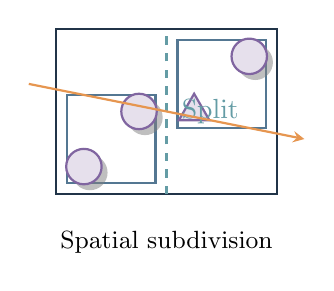
\begin{tikzpicture}[scale=0.7]
                % Scene with objects and bounding boxes
                \draw[thick, PrimaryColor] (-0.5,-0.5) rectangle (3.5,2.5);
                \draw[thick, SecondaryColor] (-0.3,-0.3) rectangle (1.3,1.3);
                \draw[thick, SecondaryColor] (1.7,0.7) rectangle (3.3,2.3);
                
                % Objects
                \node[sphere, scale=0.3] at (0,0) {};
                \node[sphere, scale=0.3] at (1,1) {};
                \node[triangle, scale=0.3] at (2,1) {};
                \node[sphere, scale=0.3] at (3,2) {};
                
                % Split line
                \draw[dashed, AccentColor, thick] (1.5,-0.5) -- (1.5,2.5);
                \node[right] at (1.6,1) {\textcolor{AccentColor}{Split}};
                
                % Ray traversal example
                \draw[ray] (-1,1.5) -- (4,0.5);
                
                \node[below] at (1.5,-1) {\small Spatial subdivision};
            \end{tikzpicture}
            
            \vspace{0.3cm}
            \begin{conceptbox}{Traversal}
                \textbf{Stack-based traversal:} Test bounding boxes, push hit children onto stack
            \end{conceptbox}
        \end{column}
    \end{columns}
\end{frame}

% --- Section 10: Hardware Acceleration ---
\section{Hardware Ray Tracing Revolution}

\begin{frame}{The Hardware Revolution}
    \begin{center}
        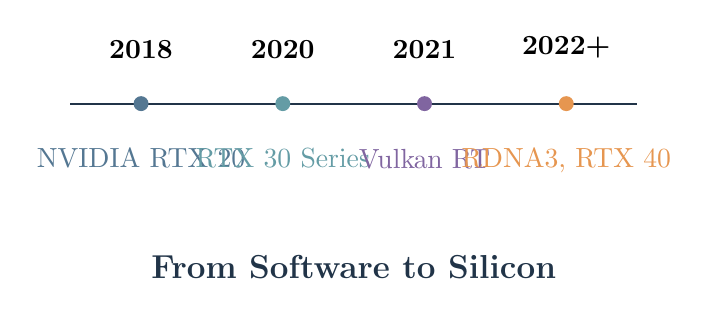
\begin{tikzpicture}[scale=0.9]
            % Timeline
            \draw[thick, PrimaryColor] (0,0) -- (8,0);
            
            % Milestones
            \node[above] at (1,0.5) {\textbf{2018}};
            \node[below] at (1,-0.5) {\textcolor{SecondaryColor}{NVIDIA RTX 20}};
            \fill[SecondaryColor] (1,0) circle (3pt);
            
            \node[above] at (3,0.5) {\textbf{2020}};
            \node[below] at (3,-0.5) {\textcolor{AccentColor}{RTX 30 Series}};
            \fill[AccentColor] (3,0) circle (3pt);
            
            \node[above] at (5,0.5) {\textbf{2021}};
            \node[below] at (5,-0.5) {\textcolor{ObjectColor}{Vulkan RT}};
            \fill[ObjectColor] (5,0) circle (3pt);
            
            \node[above] at (7,0.5) {\textbf{2022+}};
            \node[below] at (7,-0.5) {\textcolor{RayColor}{RDNA3, RTX 40}};
            \fill[RayColor] (7,0) circle (3pt);
            
            \node[below] at (4,-2) {\large \textcolor{PrimaryColor}{\textbf{From Software to Silicon}}};
        \end{tikzpicture}
    \end{center}
    
    \begin{columns}
        \begin{column}{0.5\textwidth}
            \textbf{Hardware Features:}
            \begin{itemize}
                \item Dedicated RT cores
                \item Hardware BVH traversal
                \item Triangle intersection units
                \item Tensor cores for denoising
            \end{itemize}
        \end{column}
        \begin{column}{0.5\textwidth}
            \textbf{Performance Impact:}
            \begin{itemize}
                \item 10-100x speedup over compute shaders
                \item Real-time ray tracing in games
                \item Interactive path tracing
                \item AI-accelerated denoising
            \end{itemize}
        \end{column}
    \end{columns}
\end{frame}

\begin{frame}{RTX Architecture Deep Dive}
    \begin{center}
        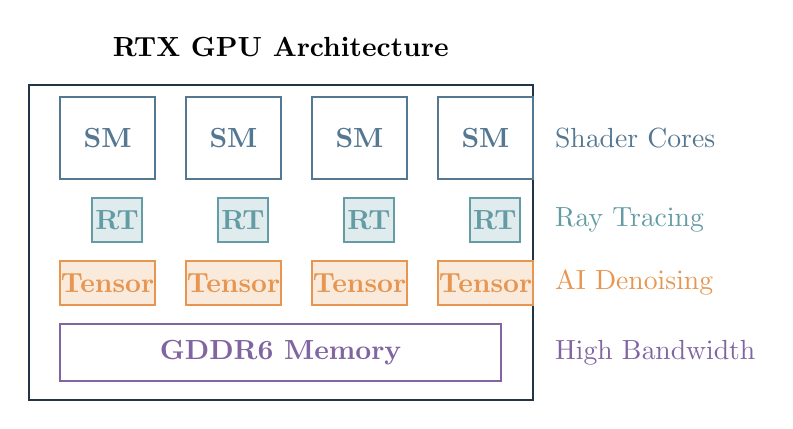
\begin{tikzpicture}[scale=0.8]
            % GPU die representation
            \draw[thick, PrimaryColor] (0,0) rectangle (8,5);
            \node[above] at (4,5.3) {\textbf{RTX GPU Architecture}};
            
            % Streaming Multiprocessors
            \foreach \x in {0.5,2.5,4.5,6.5} {
                \draw[SecondaryColor, thick] (\x,3.5) rectangle (\x+1.5,4.8);
                \node at (\x+0.75,4.15) {\textcolor{SecondaryColor}{\textbf{SM}}};
            }
            
            % RT Cores
            \foreach \x in {1,3,5,7} {
                \draw[AccentColor, thick, fill=AccentColor!20] (\x,2.5) rectangle (\x+0.8,3.2);
                \node at (\x+0.4,2.85) {\textcolor{AccentColor}{\textbf{RT}}};
            }
            
            % Tensor Cores
            \foreach \x in {0.5,2.5,4.5,6.5} {
                \draw[RayColor, thick, fill=RayColor!20] (\x,1.5) rectangle (\x+1.5,2.2);
                \node at (\x+0.75,1.85) {\textcolor{RayColor}{\textbf{Tensor}}};
            }
            
            % Memory
            \draw[ObjectColor, thick] (0.5,0.3) rectangle (7.5,1.2);
            \node at (4,0.75) {\textcolor{ObjectColor}{\textbf{GDDR6 Memory}}};
            
            % Labels
            \node[right] at (8.2,4.15) {\textcolor{SecondaryColor}{Shader Cores}};
            \node[right] at (8.2,2.85) {\textcolor{AccentColor}{Ray Tracing}};
            \node[right] at (8.2,1.85) {\textcolor{RayColor}{AI Denoising}};
            \node[right] at (8.2,0.75) {\textcolor{ObjectColor}{High Bandwidth}};
        \end{tikzpicture}
    \end{center}
    
    \begin{raybox}{RT Core Functions}
        \textbf{Hardware accelerated:} BVH traversal, ray-triangle intersection, ray-box intersection\\
        \textbf{Result:} Massive parallel ray processing with dedicated silicon
    \end{raybox}
\end{frame}

\begin{frame}{Modern Ray Tracing APIs}
    \begin{columns}
        \begin{column}{0.5\textwidth}
            \begin{conceptbox}{DirectX Raytracing (DXR)}
                \textbf{Microsoft's API:}
                \begin{itemize}
                    \item Raytracing Pipeline State Objects
                    \item Acceleration Structure builds
                    \item Ray generation/intersection/hit shaders
                    \item Widely adopted in games
                \end{itemize}
            \end{conceptbox}
            
            \vspace{0.3cm}
            \begin{conceptbox}{Vulkan Ray Tracing}
                \textbf{Cross-platform standard:}
                \begin{itemize}
                    \item VK\_KHR\_ray\_tracing\_pipeline
                    \item Lower-level control
                    \item Multi-vendor support
                    \item Mobile and desktop
                \end{itemize}
            \end{conceptbox}
        \end{column}
        \begin{column}{0.5\textwidth}
            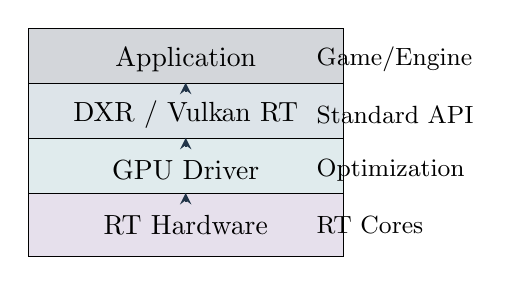
\begin{tikzpicture}[scale=0.7]
                % API stack
                \node[rectangle, draw, fill=PrimaryColor!20, minimum width=4cm, minimum height=0.8cm] (app) at (0,3) {Application};
                \node[rectangle, draw, fill=SecondaryColor!20, minimum width=4cm, minimum height=0.8cm] (api) at (0,2) {DXR / Vulkan RT};
                \node[rectangle, draw, fill=AccentColor!20, minimum width=4cm, minimum height=0.8cm] (driver) at (0,1) {GPU Driver};
                \node[rectangle, draw, fill=ObjectColor!20, minimum width=4cm, minimum height=0.8cm] (hw) at (0,0) {RT Hardware};
                
                % Arrows
                \draw[arrow] (app) -- (api);
                \draw[arrow] (api) -- (driver);
                \draw[arrow] (driver) -- (hw);
                
                % Side annotations
                \node[right] at (2.2,3) {\small Game/Engine};
                \node[right] at (2.2,2) {\small Standard API};
                \node[right] at (2.2,1) {\small Optimization};
                \node[right] at (2.2,0) {\small RT Cores};
            \end{tikzpicture}
            
            \vspace{0.5cm}
            \textbf{Key Innovation:}
            \begin{itemize}
                \item Shader-driven ray tracing
                \item Flexible hit/miss handling
                \item Integration with rasterization
                \item Real-time performance
            \end{itemize}
        \end{column}
    \end{columns}
\end{frame}

% --- Section 11: Path Tracing ---
\section{Path Tracing: The Ultimate Goal}

\begin{frame}{Beyond Ray Tracing: Path Tracing}
    \begin{center}
        \begin{tikzpicture}[scale=0.8]
            % Scene setup
            \node[circle, fill=LightColor, minimum size=1cm] (light) at (1,4) {\faIcon{sun}};
            \node[sphere] (sphere1) at (3,2) {};
            \node[sphere] (sphere2) at (5,1) {};
            \node[eye] (eye) at (7,2) {\faIcon{eye}};
            
            % Multiple path samples
            \draw[ray, bend left=10] (eye) to (sphere2);
            \draw[reflectray, bend right=15] (sphere2) to (sphere1);
            \draw[lightray, bend left=20] (sphere1) to (light);
            
            \draw[ray, bend left=20] (eye) to (sphere2);
            \draw[reflectray, bend left=10] (sphere2) to (3,4);
            \draw[lightray] (3,4) to (light);
            
            \draw[ray, bend right=10] (eye) to (sphere2);
            \draw[reflectray, bend right=25] (sphere2) to (sphere1);
            \draw[refractray, bend left=15] (sphere1) to (2,0);
            
            % Path labels
            \node[below] at (4,-0.5) {\raycolor{\textbf{Multiple Random Paths}}};
            \node[above] at (4,4.8) {\textcolor{LightColor}{\textbf{Monte Carlo Integration}}};
        \end{tikzpicture}
    \end{center}
    
    \begin{columns}
        \begin{column}{0.5\textwidth}
            \begin{raybox}{Ray Tracing Limitations}
                \begin{itemize}
                    \item Perfect mirrors only
                    \item Direct illumination focus
                    \item Limited global effects
                    \item Deterministic sampling
                \end{itemize}
            \end{raybox}
        \end{column}
        \begin{column}{0.5\textwidth}
            \begin{raybox}{Path Tracing Advantages}
                \begin{itemize}
                    \item Physically accurate lighting
                    \item Global illumination
                    \item Soft shadows, caustics
                    \item Unbiased rendering
                \end{itemize}
            \end{raybox}
        \end{column}
    \end{columns}
\end{frame}

\begin{frame}{The Rendering Equation}
    \begin{center}
        \begin{mathbox}{The Holy Grail of Computer Graphics}
            \begin{align}
                L_o(\mathbf{p}, \omega_o) = L_e(\mathbf{p}, \omega_o) + \int_\Omega f(\mathbf{p}, \omega_i, \omega_o) L_i(\mathbf{p}, \omega_i) (\mathbf{n} \cdot \omega_i) d\omega_i
            \end{align}
        \end{mathbox}
    \end{center}
    
    \begin{columns}
        \begin{column}{0.5\textwidth}
            \textbf{Components:}
            \begin{itemize}
                \item $L_o$ = Outgoing radiance
                \item $L_e$ = Emitted light
                \item $f$ = BRDF (material properties)
                \item $L_i$ = Incoming radiance
                \item $\Omega$ = Hemisphere of directions
            \end{itemize}
        \end{column}
        \begin{column}{0.5\textwidth}
            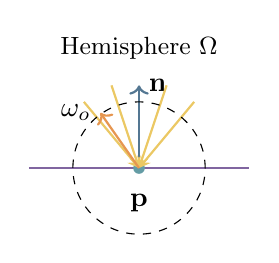
\begin{tikzpicture}[scale=0.7]
                % Surface point
                \draw[thick, ObjectColor] (-1,0) -- (3,0);
                \fill[AccentColor] (1,0) circle (3pt);
                \node[below] at (1,-0.3) {$\mathbf{p}$};
                
                % Normal
                \draw[->, SecondaryColor, thick] (1,0) -- (1,1.5);
                \node[right] at (1,1.5) {$\mathbf{n}$};
                
                % Incoming light hemisphere
                \draw[lightray] (0,1.2) -- (1,0);
                \draw[lightray] (0.5,1.5) -- (1,0);
                \draw[lightray] (1.5,1.5) -- (1,0);
                \draw[lightray] (2,1.2) -- (1,0);
                
                % Outgoing direction
                \draw[->, RayColor, thick] (1,0) -- (0.3,1);
                \node[left] at (0.3,1) {$\omega_o$};
                
                % Hemisphere
                \draw[dashed] (1,0) circle (1.2);
                \node[above] at (1,1.8) {\small Hemisphere $\Omega$};
            \end{tikzpicture}
        \end{column}
    \end{columns}
    
    \begin{conceptbox}{The Challenge}
        \textbf{Integral:} Infinite directions to sample → Monte Carlo approximation needed
    \end{conceptbox}
\end{frame}

\begin{frame}{Path Tracing vs Ray Tracing}
    \begin{center}
        \begin{tikzpicture}[scale=0.7]
            % Ray Tracing side
            \node[above] at (-2,3) {\textbf{Ray Tracing}};
            \node[eye] (eye1) at (-4,1) {};
            \node[triangle] (near1) at (-2,1.2) {};
            \node[triangle] (far1) at (-1,1) {};
            \draw[ray] (eye1) -- (-2,1.5) -- (-0.5,1.2);
            \draw[ray] (eye1) -- (-2,0.5) -- (-0.5,0.8);
            \node[below] at (-3,0.2) {\small Converging rays};
            \node[below] at (-3,-0.1) {\small Size $\propto$ 1/distance};
            
            % vs
            \node at (0,1) {\huge \textcolor{AccentColor}{vs}};
            
            % Path Tracing side
            \node[above] at (2,3) {\textbf{Path Tracing}};
            \node[eye] (eye2) at (0.5,1) {};
            \node[sphere] (obj2) at (2,1) {};
            \node[sphere] (obj3) at (3,2) {};
            \node[circle, fill=LightColor, minimum size=0.6cm] (light2) at (4,0.5) {};
            
            % Multiple random paths
            \draw[ray, bend left=10] (eye2) to (sphere2);
            \draw[reflectray, bend right=15] (sphere2) to (sphere1);
            \draw[lightray, bend left=20] (sphere1) to (light);
            
            \draw[ray, bend left=20] (eye2) to (sphere2);
            \draw[reflectray, bend left=10] (sphere2) to (3,4);
            \draw[lightray] (3,4) to (light);
            
            \draw[ray, bend right=10] (eye2) to (sphere2);
            \draw[reflectray, bend right=25] (sphere2) to (sphere1);
            \draw[refractray, bend left=15] (sphere1) to (2,0);
            
            % Path labels
            \node[below] at (4,-0.5) {\raycolor{\textbf{Multiple Random Paths}}};
            \node[above] at (4,4.8) {\textcolor{LightColor}{\textbf{Monte Carlo Integration}}};
        \end{tikzpicture}
    \end{center}
    
    \begin{columns}
        \begin{column}{0.5\textwidth}
            \begin{raybox}{Ray Tracing Limitations}
                \begin{itemize}
                    \item Perfect mirrors only
                    \item Direct illumination focus
                    \item Limited global effects
                    \item Deterministic sampling
                \end{itemize}
            \end{raybox}
        \end{column}
        \begin{column}{0.5\textwidth}
            \begin{raybox}{Path Tracing Advantages}
                \begin{itemize}
                    \item Physically accurate lighting
                    \item Global illumination
                    \item Soft shadows, caustics
                    \item Unbiased rendering
                \end{itemize}
            \end{raybox}
        \end{column}
    \end{columns}
\end{frame}

% --- Section 12: Shading Models Preview ---
\section{The Art of Shading (Preview)}

\begin{frame}{From Geometry to Beauty}
    \begin{center}
        \large \textcolor{PrimaryColor}{We've traced rays and found intersections...}\\
        \vspace{0.5cm}
        \huge \textcolor{AccentColor}{Now what color should that pixel be?}
    \end{center}
    
    \begin{columns}
        \begin{column}{0.5\textwidth}
            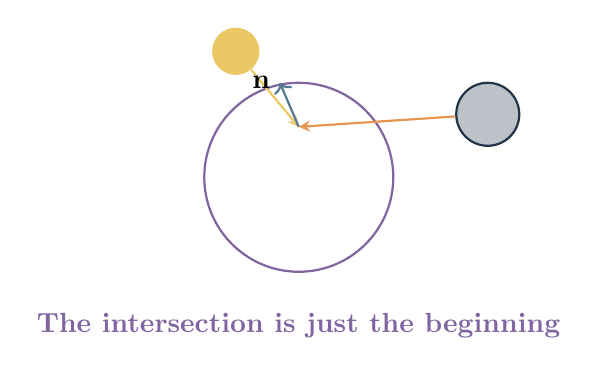
\begin{tikzpicture}[scale=0.8]
                % Simple sphere with different shading
                \draw[thick, ObjectColor] (0,0) circle (1.5);
                
                % Light direction
                \node[circle, fill=LightColor, minimum size=0.6cm] (light) at (-1,2) {};
                \draw[lightray] (light) -- (0,0.8);
                
                % Normal at surface
                \draw[->, SecondaryColor, thick] (0,0.8) -- (-0.3,1.5);
                \node[left] at (-0.3,1.5) {$\mathbf{n}$};
                
                % Eye direction
                \node[eye] (eye) at (3,1) {};
                \draw[ray] (eye) -- (0,0.8);
                
                \node[below] at (0,-2) {\textcolor{ObjectColor}{\textbf{The intersection is just the beginning}}};
            \end{tikzpicture}
        \end{column}
        \begin{column}{0.5\textwidth}
            \textbf{Shading determines:}
            \begin{itemize}
                \item Surface appearance
                \item Material properties
                \item Light interaction
                \item Visual realism
            \end{itemize}
            
            \vspace{0.5cm}
            \alert{Next lesson:} Deep dive into shading models!
        \end{column}
    \end{columns}
\end{frame}

\begin{frame}{Shading Models: A Sneak Peek}
    \begin{center}
        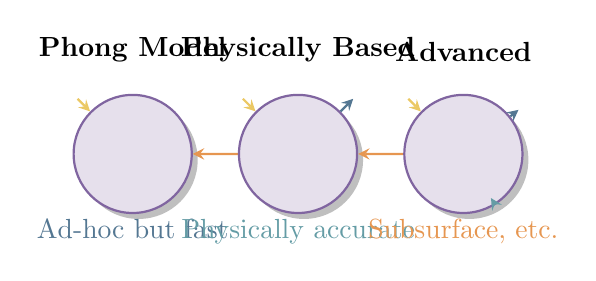
\begin{tikzpicture}[scale=0.7]
            % Phong model illustration
            \node[above] at (-3,2.5) {\textbf{Phong Model}};
            \node[sphere] (phong) at (-3,1) {};
            \draw[lightray] (-4,2) -- (phong);
            \draw[ray] (-1,1) -- (phong);
            \node[below] at (-3,0) {\textcolor{SecondaryColor}{Ad-hoc but fast}};
            
            % PBR illustration  
            \node[above] at (0,2.5) {\textbf{Physically Based}};
            \node[sphere] (pbr) at (0,1) {};
            \draw[lightray] (-1,2) -- (pbr);
            \draw[reflectray] (pbr) -- (1,2);
            \draw[ray] (2,1) -- (pbr);
            \node[below] at (0,0) {\textcolor{AccentColor}{Physically accurate}};
            
            % Advanced illustration
            \node[above] at (3,2.5) {\textbf{Advanced}};
            \node[sphere] (adv) at (3,1) {};
            \draw[lightray] (2,2) -- (adv);
            \draw[refractray] (adv) -- (3.5,0.2);
            \draw[reflectray] (adv) -- (4,1.8);
            \node[below] at (3,0) {\textcolor{RayColor}{Subsurface, etc.}};
        \end{tikzpicture}
    \end{center}
    
    \begin{columns}
        \begin{column}{0.33\textwidth}
            \begin{conceptbox}{Phong/Blinn-Phong}
                \textbf{Components:}
                \begin{itemize}
                    \item Ambient
                    \item Diffuse  
                    \item Specular
                \end{itemize}
                \textbf{Pro:} Fast, simple\\
                \textbf{Con:} Not physically accurate
            \end{conceptbox}
        \end{column}
        \begin{column}{0.33\textwidth}
            \begin{conceptbox}{Physically Based}
                \textbf{Based on:}
                \begin{itemize}
                    \item Energy conservation
                    \item Fresnel equations
                    \item Microfacet theory
                \end{itemize}
                \textbf{Pro:} Realistic, consistent\\
                \textbf{Con:} More complex
            \end{conceptbox}
        \end{column}
        \begin{column}{0.33\textwidth}
            \begin{conceptbox}{Advanced Models}
                \textbf{Features:}
                \begin{itemize}
                    \item Subsurface scattering
                    \item Volumetric effects
                    \item Layered materials
                \end{itemize}
                \textbf{Pro:} Ultimate realism\\
                \textbf{Con:} Computationally expensive
            \end{conceptbox}
        \end{column}
    \end{columns}
\end{frame}

% --- Section 13: Applications and Future ---
\section{Applications and Future}

\begin{frame}{Ray Tracing in the Real World}
    \begin{center}
        \begin{tikzpicture}[scale=0.8]
            % Applications
            \node[rectangle, rounded corners, fill=PrimaryColor!20, minimum width=2.5cm, minimum height=1.5cm] (movies) at (0,2) {Movies \& VFX};
            \node[rectangle, rounded corners, fill=SecondaryColor!20, minimum width=2.5cm, minimum height=1.5cm] (games) at (4,2) {Video Games};
            \node[rectangle, rounded corners, fill=AccentColor!20, minimum width=2.5cm, minimum height=1.5cm] (arch) at (0,0) {Architecture};
            \node[rectangle, rounded corners, fill=ObjectColor!20, minimum width=2.5cm, minimum height=1.5cm] (product) at (4,0) {Product Design};
            
            % Center
            \node[circle, fill=LightColor, minimum size=2cm] (center) at (2,1) {\textbf{Ray Tracing}};
            
            % Connections
            \draw[arrow] (center) -- (movies);
            \draw[arrow] (center) -- (games);
            \draw[arrow] (center) -- (arch);
            \draw[arrow] (center) -- (product);
            
            % Icons
            \node at (0,2.5) {\faIcon{film}};
            \node at (4,2.5) {\faIcon{gamepad}};
            \node at (0,0.5) {\faIcon{building}};
            \node at (4,0.5) {\faIcon{car}};
        \end{tikzpicture}
    \end{center}
    
    \begin{columns}
        \begin{column}{0.5\textwidth}
            \textbf{Traditional (Offline):}
            \begin{itemize}
                \item Movie rendering
                \item Architectural visualization
                \item Product design
                \item Scientific simulation
            \end{itemize}
        \end{column}
        \begin{column}{0.5\textwidth}
            \textbf{Modern (Real-time):}
            \begin{itemize}
                \item RTX graphics cards
                \item Video games
                \item VR/AR applications
                \item Interactive design
            \end{itemize}
        \end{column}
    \end{columns}
\end{frame}

\begin{frame}{The Future is Bright}
    \begin{conceptbox}{Hardware Acceleration}
        \textbf{Modern GPUs:} Dedicated ray tracing cores, massive parallelization
    \end{conceptbox}
    
    \vspace{0.3cm}
    
    \begin{columns}
        \begin{column}{0.5\textwidth}
            \textbf{Emerging Techniques:}
            \begin{itemize}
                \item Machine learning denoising
                \item Hybrid rendering
                \item Path tracing
                \item Photon mapping
            \end{itemize}
        \end{column}
        \begin{column}{0.5\textwidth}
            \textbf{New Applications:}
            \begin{itemize}
                \item Medical imaging
                \item Autonomous vehicles
                \item Metaverse platforms
                \item Scientific visualization
            \end{itemize}
        \end{column}
    \end{columns}
    
    \vspace{0.5cm}
    
    \begin{center}
        \large \textcolor{PrimaryColor}{\textbf{Ray tracing is becoming the future of computer graphics!}}
    \end{center}
\end{frame}

% --- Conclusion ---
\section{Wrapping Up}

\begin{frame}{Key Takeaways}
    \begin{enumerate}
        \item \highlight{Ray tracing simulates light transport} by reversing the natural process
        \item \highlight{Mathematical foundation} involves solving intersection equations for different geometric primitives
        \item \highlight{Secondary rays} enable realistic effects like reflections, refractions, and shadows
        \item \highlight{Implementation challenges} include floating-point precision and performance optimization
        \item \highlight{Real-world impact} spans from Hollywood movies to real-time gaming
    \end{enumerate}
    
    \vspace{0.5cm}
    
    \begin{center}
        \begin{tikzpicture}[scale=0.6]
            % Final illustration
            \node[eye] (eye) at (0,0) {\faIcon{eye}};
            \node[sphere] at (2,0) {};
            \node[sphere] at (3,1) {};
            \node[triangle] at (4,-1) {};
            \node[circle, fill=LightColor, minimum size=0.8cm] at (2,2) {\faIcon{lightbulb}};
            
            \draw[ray] (eye) -- (2,0) -- (4,1);
            \draw[reflectray] (2,0) -- (3,1);
            \draw[shadowray] (2,0) -- (2,2);
            \draw[refractray] (2,0) -- (4,-1);
            
            \node[below] at (2,-2) {\textcolor{PrimaryColor}{\textbf{The art and science of light}}};
        \end{tikzpicture}
    \end{center}
\end{frame}
\end{document}